%%%%%%%%%%%%%%%%%%%%%%%%%%%%%%%%%%%%%%%%%
% Short Sectioned Assignment
% LaTeX Template
% Version 1.0 (5/5/12)
%
% This template has been downloaded from:
% http://www.LaTeXTemplates.com
%
% Original author:
% Frits Wenneker (http://www.howtotex.com)
%
% License:
% CC BY-NC-SA 3.0 (http://creativecommons.org/licenses/by-nc-sa/3.0/)
%
%%%%%%%%%%%%%%%%%%%%%%%%%%%%%%%%%%%%%%%%%

%----------------------------------------------------------------------------------------
%	PACKAGES AND OTHER DOCUMENT CONFIGURATIONS
%----------------------------------------------------------------------------------------

\documentclass[paper=a4, fontsize=11pt]{scrartcl} % A4 paper and 11pt font size

\usepackage[T1]{fontenc} % Use 8-bit encoding that has 256 glyphs
\usepackage[ngerman]{babel}
\usepackage{fourier} % Use the Adobe Utopia font for the document - comment this line to return to the LaTeX default
\usepackage{amsmath,amsfonts,amsthm} % Math packages
\usepackage{graphicx}
\usepackage[utf8]{inputenc}
\usepackage{listings}
\usepackage[section]{placeins}
\usepackage{lipsum} % Used for inserting dummy 'Lorem ipsum' text into the template
\usepackage{float}
\usepackage{multicol}

\usepackage{sectsty} % Allows customizing section commands
\allsectionsfont{\centering \normalfont\scshape} % Make all sections centered, the default font and small caps

\usepackage{fancyhdr} % Custom headers and footers
\pagestyle{fancyplain} % Makes all pages in the document conform to the custom headers and footers
\fancyhead{} % No page header - if you want one, create it in the same way as the footers below
\fancyfoot[L]{} % Empty left footer
\fancyfoot[C]{} % Empty center footer
\fancyfoot[R]{\thepage} % Page numbering for right footer
\renewcommand{\headrulewidth}{0pt} % Remove header underlines
\renewcommand{\footrulewidth}{0pt} % Remove footer underlines
\setlength{\headheight}{13.6pt} % Customize the height of the header

\numberwithin{equation}{section} % Number equations within sections (i.e. 1.1, 1.2, 2.1, 2.2 instead of 1, 2, 3, 4)
\numberwithin{figure}{section} % Number figures within sections (i.e. 1.1, 1.2, 2.1, 2.2 instead of 1, 2, 3, 4)
\numberwithin{table}{section} % Number tables within sections (i.e. 1.1, 1.2, 2.1, 2.2 instead of 1, 2, 3, 4)

\setlength\parindent{0pt} % Removes all indentation from paragraphs - comment this line for an assignment with lots of text

%----------------------------------------------------------------------------------------
%	TITLE SECTION
%----------------------------------------------------------------------------------------

\newcommand{\horrule}[1]{\rule{\linewidth}{#1}} % Create horizontal rule command with 1 argument of height

\title{	
\normalfont \normalsize 
\textsc{Karlsruhe Institute of Technology} \\ [25pt] % Your university, school and/or department name(s)
\horrule{0.5pt} \\[0.4cm] % Thin top horizontal rule
\huge Maschinelles Lernen I\\ % The assignment title
\horrule{2pt} \\[0.5cm] % Thick bottom horizontal rule
}

\author{Manuel Lang} % Your name

\date{\normalsize\today} % Today's date or a custom date

\DeclareMathOperator*{\argmax}{arg\,max}
\DeclareMathOperator*{\argmin}{arg\,min}

\begin{document}

{\small\tableofcontents}
\newpage

\maketitle % Print the title

%----------------------------------------------------------------------------------------
%	PROBLEM 1
%----------------------------------------------------------------------------------------

\section{Einführung}

\subsection{Definition Maschinelles Lernen}

Ein System lernt aus Erfahrung E in Hinblick auf eine Klasse von Aufgaben T und einem Performanzmaß P, wenn seine Leistungen bei Aufgaben aus T gemessen mit P durch Erfahrung aus E steigt.

\subsection{Komponenten eines lernenden Systems}

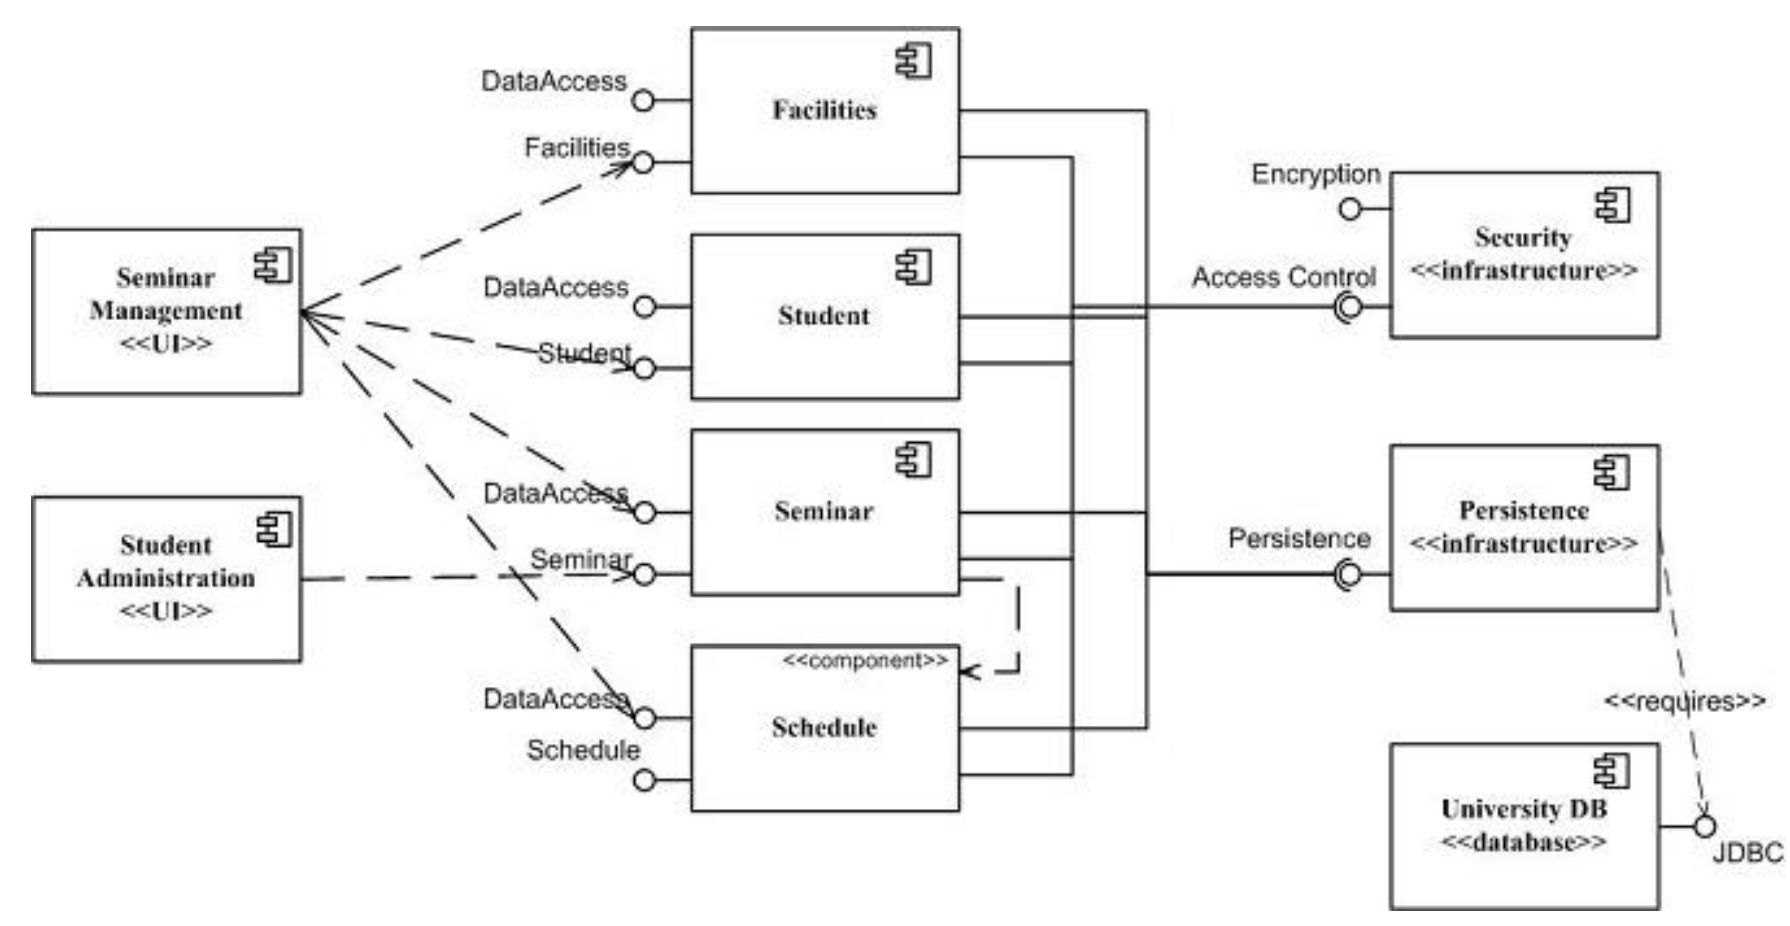
\includegraphics[width=0.7\textwidth]{/Users/Manu/Desktop/komponenten.png}

\subsection{Einordnungskriterien von Lernverfahren}

\includegraphics[width=0.7\textwidth]{/Users/Manu/Desktop/krit.png}

\section{Induktives Lernen}

Was ist Induktion? - Prozess des plausiblen Schließens vom Speziellen zum Allgemeinen

\subsection{Induktion vs Deduktion}

\begin{minipage}{.5\textwidth}
Induktion
\begin{itemize}
\item Wahrheitserweiternd
\item Macht Lebewesen überlebensfähig
\item Plausibilität
\end{itemize}
\end{minipage}% This must go next to `\end{minipage}`
\begin{minipage}{.5\textwidth}
Deduktion
\begin{itemize}
\item Wahrheitserhaltend
\item Logischer Schluss
\item Korrektheit
\end{itemize}
\end{minipage}

Induktive Lernhypothese: Jede Hypothese, die die Zielfunktion über einer genügend großen Menge von Trainingsbeispielen gut genug approximiert, wird die Zielfunktion auch über unbekannten Beispielen gut approximieren.

\subsection{Konzeptlernen als Suche im Hypothesenraum}

Konzept
\begin{itemize}
\item Beschreibt Untermenge von Objekten oder Ereignissen definiert auf größerer Menge
\item Bool'sche Funktion definiert über größere Menge
\item Beispiel: vogel: Tiere $\rightarrow$ \{true,false\}, vogel(Storch) = true, vogel(Hase) = false
\end{itemize}

Lernen von Konzepten
\begin{itemize}
\item Gegeben: Beispiele, die als Mitglieder oder Nichtmitglieder eines Konzeptes gekennzeichnet sind
\item Gesucht: Automatischer Schluss auf die Definition des zugrundeliegenden Konzepts
\item Definition Konzeptlernen: Schließen auf eine Boolean-wertige Funktion aus Trainingsbeispielen ihres Inputs und Outputs
\end{itemize}

Konsistenz und Vollständigkeit im Hypothesenraum
\begin{itemize}
\item Konsistenz: Keine negativen Beispiele werden positiv klassifiziert
\item Vollständigkeit: Alle positiven Beispiele werden als positiv klassifiziert
\end{itemize}

Lernen als Suche im Hypothesenraum
\begin{itemize}
\item Repräsentation der Hypothesen legt implizit Hypothesenraum fest (Domänenwissen -> Bias)
\item Lernen als Suche im Raum der mögliches Hypothesen: 96 mögl. Instanzen, 973 mögl. Hypothesen
\item Jeder Beschreibungsraum für Konzepte ist nach Generalität (halb-)geordnet:
\begin{itemize}
\item $h_1 = <sonnig,?,?,stark,?,?>$
\item $h_2 = <sonnig,?,?,?,?,?>$
\item $h_k$ spezieller $h_i$ <=> $\forall x \in X: [h_k(x) = 1 => h_i(x) = 1]$
\item wobei $h(x) = 1$ bedeutet: $x$ erfüllt die Hypothese $h$
\end{itemize}
\end{itemize}

\subsection{Specific-to-general-Suche}

Suche vom Speziellen zum Allgemeinen:
\begin{itemize}
\item Ausgangspunkt ist die speziellste Hypothese $<\#,...,\#>$
\item Positive Beispiele: (minimale) Verallgemeinerung
\item Negative Beispiele: werden nicht betrachtet
\end{itemize}

\begin{itemize}
\item Initialisiere h mit der spezifischten Hypothese in H
\item Für jedes positive Trainingsbeispiel x: Für jede Attributeinschränkung $a_i $ in $h = <a_0,...,a_n>$
\begin{itemize}
\item Wenn $a_i$ von $x$ erfüllt wird dann tue nichts
\item Sonst ersetze $a_i$ durch die nächstallgemeinere Einschränkung, die durch $x$ erfüllt wird
\end{itemize}
\item Gib die Hypothese aus
\end{itemize}

Beurteilung:
\begin{itemize}
\item Wichtiges Prinzip im Konzeptlernen
\item Für Hypothesenräume, die durch Konjunktionen von Attributeinschränkungen beschrieben sind garantiert das Verfahren die spezifischte Hypothese, die mit den positiven Trainingsbeispielen vereinbar ist
\item Endhypothese ist auch mit negativen Trainingsbeispielen konsistent, solange die Trainingsbeispiele korrekt sind und die Zielhypothese in H enthalten ist
\item Offene Fragen: Sind die Trainingsbeispiele konsistent? Endkonzept = korrektes Zielkonzept? Warum spezifischte Hypothese?
\end{itemize}

\subsection{Versionsraum (Version Space)/Candidate-Elimination-Algorithmus}

Versionsraum (Version Space): Der Versionsraum $VS_{H,D}$ bezüglich es Hypothesenraums $H$ und der menge von Trainingsbeispielen $D$ ist die Untermenge der Hypothesen von H, die mit den Trainingsbeispielen in D konsistent ist.\\ 
Version Space / Candidate-Elimination-Algorithmus
\begin{itemize}
\item Lernen ist inkrementell: Menge der konsistenten Hypothesen (Version space) ist ein Intervall in der partiellen Ordnung spezifischer als auf dem Hypothesenraum
\item Gespeichert werden: Menge der spezifischen Hypothesen S und Menge der allgemeinsten Hypothesen G, die alle Bereiche abdecken => Hypothesen müssen nicht einzeln gespeichert werden
\item Spezifischte und Allgemeinste Hypothesen:
\begin{itemize}
\item S = \{s | s ist eine Hypothese, die mit den betrachteten Beispielen konsistent ist und es gibt keine Hypothese, die spezifischer als s und auch konsistent mit allen Beispielen ist\}
\item Initialisierung: S = \{\#\}
\item G = \{g | g ist eine Hypothese, die mit den betrachteten Beispielen konsistent ist, und es gibt keine Hypothese, die allgemeiner als g und auch konsistent mit allen Beispielen ist\} 
\item Initialisierung: G=\{?\}
\end{itemize}
\item Ist $n$ ein negatives Beispiel
\begin{itemize}
\item Lösche aus S die Hypothesen, die n abdecken.
\item Spezialisiere die Hypothesen in G soweit, dass sie n nicht abdecken und dass sie allgemeiner als eine Hypothese in S bleiben.
\item Lösche aus G alle Hypothesen, die spezifischer als eine andere Hypothese aus G sind.
\end{itemize}
\item Ist p ein positives Beispiel
\begin{itemize}
\item Lösche aus G die mit p inkonsistenten Hypothesen.
\item Verallgemeinere die Hypothesen in S soweit, dass sie p abdecken und dass sie spezifischer als eine Hypothese in G bleiben.
\item Lösche aus S alle Hypothesen, die allgemeiner als eine andere Hypothese aus S sind.
\end{itemize}
\end{itemize}

\includegraphics[width=0.7\textwidth]{/Users/Manu/Desktop/eintvs.png}

Beurteilung
\begin{itemize}
\item Version Space konvergiert zur korrekten Hypothese (S=G)
\begin{itemize}
\item Vorraussetzung: Beispiele konsistent, korrekte Hypothese in Hypothesenraum enthalten
\item Probleme: fehlerbehaftete Trainingsdaten (Rauschen), Zielkonzept nicht von Hypothesenrepräsentation abgedeckt => mögliche Erweiterung: disjunktive Begriffe
\end{itemize}
\item Anfrage des Konzeptlerners möglichst so, dass Hypothesen im Version Space halbiert werden, dann: schnelle Lernrate / geringe Anzahl von Beispielen
\item Umgang mit teilweise gelernten Konzepten nötig
\item Wenn mehr als eine Hypothese im Versionsraum vorhanden ist dann alle klassifizieren positiv bzw. negativ => Entscheidung klar, ansonsten Mehrheitsentscheidung evtl. mit Angabe von Konfidenz, probabilistische Entscheidung / Wahrscheinlichkeit, Plausibilitätsbetrachtungen 
\item - konsistente Beispiele notwendig
\item - Attributgeneralisierungsregeln maßgebend für Lernerfolg
\item + Kein Speichern aller Beispiele notwendig
\item + Stellt fest, wann genügend Beispiele gegeben wurden (S=G)
\item Unter Umständen Art noch benötigter Beispiele erkennbar
\end{itemize}

\subsection{Notwendigkeit von Vorzugskriterien}

\begin{itemize}
\item Problem: Zielkonzept evtl. nicht im Hypothesenraum enthalten
\item Lösung: Hypothesenraum, der alle möglichen Hypothesen enthält?
\item Grundlegende Eigenschaft von induktiver Interferenz: Ein induktives Lernsystem, das keine a-priori Annahmen über die Identität des Zielkonzeptes macht, hat keine rationale Basis, um unbekannte Instanzen zu klassifizieren.
\item Induktives lernen erfordert Vorannahmen (inductive bias)
\end{itemize}

Vergleich induktiver Lernsysteme anhand ihres inducte bias
\begin{itemize}
\item Auswendiglerner: keine Vorannahme
\item Version Space: Zielkonzept kann im Hypothesenraum repräsentiert werden
\item Specific to General-Lerner: wie Version Space und zusätzlich: alle Instanzen sind negative Instanzen, solange nicht das Gegenteil bekannt ist
\item Je strenger die Vorannahmen, desto mehr unbekannte Beispiele können klassifiziert werden
\end{itemize}

Vorzugskriterien (Bias)
\begin{itemize}
\item Bias (Vorzugskriterium): Vorschrift nach der Hypothesen gebildet werden
\item Mögliche Vorzugskriterien: Verständlichkeit (für den menschlichen Benutzer), Klassifikationsgenauigkeit, Messaufwand für die verwendeten Deskriptoren, Berechnungs- und Speicheraufwand für die Hypothese
\item Hypothesenraumbias: h gehöre zu einem beschränkten Raum von Hypothesen, logische Konjunktionen, lineare Schwellwertfunktionen, Geraden, Polynome, 3-NN (Nearest Neighbor),...
\item Präferenzbias: Ordnung auf dem Raum der Hypothesen, wähle h mit der höchsten Präferenz: bevorzuge Hypothesen mit weniger Disjunktionen, bevorzuge kleinere Entscheidungsbäume
\item Problem: Es existiert keine Funktion h, die konsistent mit allen Trainingsbeispielen ist, z.B. wegen verrauschter Trainingsdaten
\item Unterschiedliche Ansätze möglich -> unterschiedliche Lösungen
\item Anpassen ddes Hypothesenraumbias: Problem, da zwar sehr gute Klassifikation i.a. durch eine komplexe Hypothese erreicht wird aber Overfitting
\item Anpassen des Präferenzbias: Wähle das h, das möglichst viele Beispiele richtig klassifiziert, Misklassifikation muss in Kauf genommen werden
\end{itemize}

\section{Unüberwachte Lernverfahren}

\subsection{k-means Clustering}

\begin{itemize}
\item klassifiziert eine Datenmenge in eine a-priori vorgegebene Anzahl von Ballungen
\item Grundidee
\begin{itemize}
\item Definieren eines Mittelpunkts für jeden Cluster
\item Iterative Anpassung / Verbesserung
\item Optimalitätskriterium: Minimierung der Abstände aller Datenpunkte von ihrem Ballungsmittelpunkt
\end{itemize}
\item Gegeben: Menge X von unklassifizierten Trainingsbeispielen mit jeweils d Attributen $x_i = < attr1_i, attr2_i, ..., attrd_i>$ und Anzahl der gesuchten Ballungen $k$
\item Gesucht: Einteilung der Trainingsmenge in Ballungen $X_1,...,X_k$ (mit Zentren $c_1,...,c_k)$ unter Minimierung von $\sum\limits_{j=1}^k \sum\limits_{x_i \in X_j} |x_i - c_j|$
\item Algorithmus
\begin{itemize}
\item Platziere k Punkte $c_j$ im d-dimensionalen Raum als initiale Mittelpunkte der Ballungen
\item Klassifiziere jedes $x_i$ gemäß der $c_j$ neu bis sich die $c_j$ nicht mehr ändern\\ $ l = arg min_{j=1}^k |x_i-c_j| \Rightarrow x_i \in X_l$\\ 
und berechne die Mittelpunkte $c_j$ zu jeder Ballung neu\\ $c_j = \frac{\sum\limits_{i=1}^{|X_j|}x_i}{|X_j|}$
\end{itemize}
\item Resultate hängen stark von der initialen Belegung der $c_j$ ab: mehrere suboptimale Lösungen möglich, mögliche Lösung: Algorithmus mehrfach mit unterschiedlichen Startpunkten
\item Resultate abhänging von der Metrik
\item Resultate abhängig von Wahl von k -> Anstoß mit mehreren k, aber Overfitting
\end{itemize}

\subsubsection{Fuzzy-k-means-Clustering}

\begin{itemize}
\item bisher: jeder Datenpunkt in genau einem Cluster
\item Abschwächung: jeder Datenpunkt hat eine abgestufte Zugehörgitkeit zu jedem Cluster
\item Problem: Laufzeit O(kn) je Iteration
\end{itemize}

\subsubsection{Einordnung k-means-Clustering}

\includegraphics[width=0.7\textwidth]{/Users/Manu/Desktop/einteilungkmeans.png}

\subsection{Hierarchisches Clustering}

\begin{itemize}
\item k-means: flache Datenbeschreibung
\item Ballungen können Subballungen und Subsubballungen haben
\item Idee: Iteratives Vereinen von (Sub-)Clustern zu größeren Clustern
\end{itemize}

\subsubsection{Agglomerative Hierarchical Clustering}

\begin{itemize}
\item Suche und verbinde zwei nächste Cluster
\item einfaches Verfahren
\item besser wenn k nicht bekannt, aber gewisse Aussagen über die Form der Cluster getroffen werden können
\item unabhängig von Initialwerten
\item finden der richtigen Parameter nötig
\item rauschanfällig
\end{itemize}

\includegraphics[width=0.7\textwidth]{/Users/Manu/Desktop/einteilungahc.png}

\subsection{Begriffliche Ballungen \& COBWEB}

Klassische Ballungsverfahren
\begin{itemize}
\item Definition der Ähnlichkeit auf der Basis einer meist numerischen Ähnlichkeitsfunktion
\item Ähnlichkeitsmaß ist kontextfrei, d.h. unabhängig von Umgebung
\item keine Ausnutzung konzeptueller Zusammenhänge
\item keine Verwendung von Gesalteigenschaften
\item Ähnlichkeit hängt nicht von der Einfachheit der resultierenden Beschreibungen ab
\end{itemize}

Bildung von Begriffshierarchien
\begin{itemize}
\item Ziel: Wie können Beispiele in Klassen bezüglich ihrer Ähnlichkeit geordnet werden? Klasseninformationen sind nicht gegeben.
\item Beispielhafte Algorithmen: COBWEB (Lernen von Begriffen für Attribute mit symbolischen Wertebereichen), CLASSIT (Lernen von Begriffen für Attribute mit numerischen Wertebereichen)
\end{itemize}

\subsubsection{COBWEB}

\begin{itemize}
\item Lernen durch inkrementelles Aufbauen und Anpassen eines Strukturbaums
\item Repräsentation der Begriffshierarchie als Baum (Verzweigungen stehen für Einteilungen der Unterbäume in verschiedene Kategorien, Bläter sind die speziellsten Begriffe)
\item Es werden nominale Attributwerte gestattet
\item Auswahl geeigneter Kategorien
\begin{itemize}
\item Maß für die Ballungsnützlichkeit (category utility)
\item Eine Ballung $c_i$ besitzt eine hohe Nützlichkeit, wenn man 
\begin{itemize}
\item falls $x$ zu $c_i$ gehört, die Attributwerte von $x$ mit hoher Wahrscheinlichkeit vorhersagen kann ($p(v|c)$) und
\item falls die Attributwerte $v$ von $x$ gegeben sind, die Zugehörigkeit von $x$ zu $c_i$ mit hoher Wahrscheinlichkeit bestimmt werden kann ($p(c|v)$)
\end{itemize}
\end{itemize}
\item Maximiere die Ähnlichkeit zwischen den Instanzen einer Klasse und gleichzeitig die Unterschiede zwischen den Klassen
\item Man erhält ein Maß für die Vorhersagekraft und die Vorhersagbarkeit jedes Attributes in einem Konzept (Category Utility)\\ 
$CU = \sum\limits_{k=1}^{K} \sum\limits_{i=1}^I \sum\limits_{j=1}^{J(i)} P(A_i = V_{ij}) \cdot P(A_i = V_{ij} | C_k) \cdot P(C_k|A_i = V_{ij})$\\ 
$C_1,...,C_k$ = Partitionierung in Unterkonzepte, $K$ = Anzahl der Klassen (Nachfolgeknoten), $I$ = Anzahl der Attribute, $J(i)$ = Anzahl der Attributwerte des i-ten Attributes, $V_{ij}$ = j-ter möglicher Wert für Attribut i, $P(A_i=V_{ij} | C_k)$ = Vorhersagbarkeit (predictability) eines Attributwertes, $P(C_k|A_i = V_{ij})$ = Vorhersagekraft (predictiveness) eines Attributwertes
\end{itemize}

\includegraphics[width=0.7\textwidth]{/Users/Manu/Desktop/einteilungcw.png}

\section{Lerntheorie, Algorithmenunabhängige Verfahren (für überwachtes induktives Lernen)}

\subsection{Definition Lernmaschine}

\begin{itemize}
\item Eine lernende Maschine wird bestimmt durch:
\begin{itemize}
\item Hypothesenraum {$h_\alpha : \alpha \in A$}
\item Lernverfahren: die Methode um $\alpha_{opt}$ mit Hilfe von Lernbeispielen zu finden (benötigt Fehlerfunktion, Optimierungsmethode)
\end{itemize}
\item Das resultierende (Entscheidungs-) Modell $M_{opt}$ ist gegeben durch die Auswertung der optimalen Hypothese $h_{\alpha_{opt}}$, die durch die lernende(n) Maschine(n) bestimmt wird
\item Problem: Welche Maschine ist zu wählen (Welches Lernverfahren?) Welches Modell soll gewählt werden?
\end{itemize}

\subsection{Probleme beim Lernen}

\begin{itemize}
\item Statistisches Problem: Das Verfahren betrachtet einen - gemessen an der Menge von Trainingsdaten - \glqq zu großen \grqq\ Hypothesenraum (auf Basis der Trainingsdaten eignen sich mehrere Hypothesen gleichermaßen gut)
\item Komplexitätsproblem: Aufgrund der Komplexität des Problems kann das Lernverfahren nicht das Finden einer optimalen Lösung innerhalb des Hypothesenraumes garantieren. (Bei Verwendung von speziellen Verfahren oder Heuristiken besteht die Gefahr einer suboptimalen Lösung)
\item Repräsentationsproblem: Der Hypothesenraum enthält keine ausreichend gute Approximationen der Zielfunktion/Konzept etc... (Das Lernverfahren kann einen gewünschten Approximationsgrad nicht liefern.)
\end{itemize}

\subsection{Überwachtes Lernen aus Beispielen}

Lernen = Schätzen einer Abbildung (Hypothese) $h_\alpha(\vec{x}) = y$ mit Hilfe von (bekannten) Beispielen (Lernbeispielen) $(\vec{x_1}, y_1) ... (\vec{x_n},y_n) \in X \times Y$ generiert von einem (nicht bekannten) System mit der Wahrscheinlichkeit $P(\vec{x},y)$

\subsection{Fehler: empirischer \& realer Fehler}

Der reale Fehler $E(h) = \int l(h(\vec{x}),y)dP(\vec{x},y)$ bezüglich aller real vorkommenden Daten ist leider nicht berechenbar -> gute Schätzung nötig.\\ 
Empirischer Fehler $E_D(h) = \frac{1}{|D|} \sum\limits_{(\vec{x},y) \in D} l(h(\vec{x}),y)$

Fehlerminimierung durch Gradientenabstieg

\subsection{Overfitting}

\begin{itemize}
\item Definition: Die Tendenz der Maschine sich beim Lernen auf die Lernbeispiele zu spezialisieren (auswendig lernen)
\item Formal: $h \in H - overfit = \exists h' \in H s.d. \forall Testdaten E_{Lerndaten}(h) < E_{Lerndaten}(h') \and E_{Testdaten}(h) > E_{Testdaten}(h')$
\item Lernfehler fällt, Testfehler steigt, Generalisierung fällt
\item Erklärung: Lerndatenmenge und Testdatenmenge unterschiedlich (je nach Komplexität der Hypothese) -> unterschiedlicher Verlauf von $E_{Lern}(h)$ und $E_{Verfifikation}(h)$
\item Lösung: Repräsentative Beispiele (Anzahl und Art/Verteilung), Lernprozess durch den Verifikationsfehler steuern (Verifikationsdatensatz kann anschließend nicht für die Gütebestimmung genutzt werden), richtige Wahl und Suche der optimalen Hypothesen $h_a$
\end{itemize}

\subsection{Modellauswahl (Crossvalidation, Bootstrap, AdaBoost)}

\begin{itemize}
\item Cross-Validierung
\begin{itemize}
\item Teile die Daten wiederholt in Lern- und Validierungsdaten
\item Bestimme darauf verschiedene Hypothesen (bzw. deren Parameter)
\item Berechne jeweils Generalisierung
\item Wiederhole
\end{itemize}
\item n-fold-crossvalidation
\begin{itemize}
\item Zerlege die Menge der Lerndaten in n Mengen
\item Trainiere jew. auf n-1 Mengen, teste auf 1 Menge
\item Wiederhole
\end{itemize}
\item Leave One Out (Spezialfall)
\begin{itemize}
\item Jeweils ein Beispiel für das Lernen weglassen
\item Addiere Fehler für weggelassene Beispiele
\item Wiederhole
\end{itemize}
\item statistische Auswertung (Mittelwert, Varianz, ...) auf verschiedenen Modellen auch mit relativ wenig Lerndaten evaluieren
\end{itemize}

Bootstrap
\begin{itemize}
\item Grundgedanke: Wie kann man mit einfachen Verfahren mehr erreichen?
\item In der Literator oft - allgemeiner anekdotischer Hintergrund
\begin{itemize}
\item Baron Münchhausen: am eigenen Schopf aus dem Sumpf gezogen
\item (für Informatiker) Computer startet zunächst ein einfaches Programm um dann vereinfachte Programme zu starten -> mächtige Leistung
\end{itemize}
\item und beim Lernen
\begin{itemize}
\item Ziehe zufällig (mit Zurücklegen) aus D jeweils |D| Beispiele m Mal
\item Bestimme jeweils die Modell-Parameter
\item Wiederhole
\item Bestimme den Mittelwert, Varianz,... der Parameter des Modells
\end{itemize}
\item Analyse der Güte/Stabilität
\item mit weiteren Ansätzen höhere Güte des Modells erreichen
\end{itemize}

Bagging (Bootstrap aggregation)
\begin{itemize}
\item Variante des Bootstrap
\item Verwende mehrere Modelle mit Bootstrap-Prinzip
\item ziehe $n < |D|$ Beispiele mit Zurücklegen
\item Bestimme die jeweiligen Modelle
\item Kombinieren die Modelle z.B. durch gewichtete Summe
\item Höhere Güte des Modells
\item Aussagen über die Stabilität des Modells (große Abweichungen in den einzelnen Modellen = instabil)
\end{itemize}

Boosting/AdaBoost aus CV bekannt

\subsection{Was ist PAC (Lernbarkeit)?}

PAC = Probably Approximate Correct\\ 
Gegeben: 
\begin{itemize}
\item eine Menge X von Instanzen der Länge n
\item ein Konzept C
\item ein Hypothesenraum H
\item eine Lerndatenmenge D
\end{itemize}

Kann eine korrekte Hypothese aus $H, h(\vec{x}) = c(\vec{x}), \forall \vec{x} \in D$ gefunden werden?
\begin{itemize}
\item Nein
\item aber eine $\epsilon$-genaue: $E_D(h) \le \epsilon, 0 \le \epsilon \le \frac{1}{2}$
\item Approximate Correct
\end{itemize}

Kann diese sicher gefunden werden?
\begin{itemize}
\item Nein
\item aber mit beliebiger Wahrscheinlichkeit $1-\delta, 0<\delta<\frac{1}{2}$
\item Probably
\end{itemize}

Wie ist das Problem (Finden der Hypothese) lösbar?
\begin{itemize}
\item in polynomialer Zeit abh. von $\frac{1}{\delta}, \frac{1}{\epsilon},n$
\item mit Speicheraufwand abh. von: $C$
\end{itemize}

Und die Anzahl der benötigten Lerndaten (Stichprobenkomplexität) ist: $m \ge \frac{1}{\epsilon}(ln(\frac{1}{\delta})+ln|H|)$\\ 
Und was heißt das?
\begin{itemize}
\item je größer die gewünschte Sicherheit
\item je kleiner der zulässige Fehler
\item je größer der Hypothesenraum
\item um so größer die Anzahl der benötigten Daten
\end{itemize}

\subsection{Approximation des realen Fehlers nach Vapnik und Chervonenkis}

\begin{itemize}
\item Vapnik-Chervonenskis (VC) Dimensionen: Die VC Dimensionen von $H^\alpha$
 (Hypothesenraum) ist gleich der maximalen Anzahl von Datenpunkten (aus einer Menge $S$) die von $H^\alpha$ beliebig separiert weren
\item Eine Abbildung (Hypothese) $h$ separiert die Daten aus $S$ wenn durch $h$ zwei Untermengen definiert werden ${x|h(x)=0}$ und ${x|h(x)=1}$
\item $VC(h) =$ Maß für die Kapazität von lernenden Maschinen
\end{itemize}

Abschätzung des Testfehlers
\begin{itemize}
\item Nach Vapnik gilt mit Wahrscheinlichkeit $1-\eta$: $E(h_\alpha) \le \approx E_{emp}(h_\alpha) + \sqrt{... \frac{VC(h_\alpha)}{N}...}$ mit VC-Dimensionen der lernenden Maschine $VC(h_\alpha)$, Anzahl der Lernbeispiele $N$, empirischem Fehler abhängig von $VC(h_\alpha)$ und $N$ $E_{emp}(h_\alpha)$ und realem (zu minimierenden) Fehler $E(h_\alpha)$
\item Lernerfolg ist abhängig von:
\begin{itemize}
\item Kapazität der lernenden Maschine (so gering wie nötig)
\item Optimierungsmethode (so gut wie möglich)
\item Lernbeispiele (repräsentativ, so viele wie möglich)
\end{itemize}
\end{itemize}

\subsection{Wie kann korrektes Lernen erfolgen?}

\subsubsection{Structural Risk Minimization}

Ziel: finde eine Lösung für\\ $min_{H_n}E_{emp}(h_\alpha) + \sqrt{... \frac{VC(h_\alpha)}{N}...}) \rightarrow$ finde $VC(h_\alpha) (\glqq Maschine \grqq)$, $N$ (\glqq Beispiele \grqq) und $a$ (\glqq Minimum des emp. Fehlers\grqq)\\ 
Ideale Lösung
\begin{itemize}
\item Minimiere Summe (nicht Summanden)
\item Strukturiere den Hypothesenraum
\item Suche Optimum (Minimum für $E(h_\alpha)$)
\end{itemize}

Probleme
\begin{itemize}
\item Strukturierung
\begin{itemize}
\item Berechnung der VC Dimension schwer, rechenintensiv, für viele Hypothesenraäume unmöglich
\end{itemize}
\item Optimierung
\begin{itemize}
\item Finden, definieren der Hypothesenräume
\item große Kapazität $\rightarrow$ kleiner empirischer Fehler
\item geringe Kapazität $\rightarrow$ größerer Fehler
\item Minimierung von $E_{emp}(h_\alpha^n)$, $\forall H^n$
\end{itemize}
\end{itemize}

\section{Reinforcement Learning}

\begin{itemize}
\item Problemstellung: Markov decision process (MDP)
\item Lernziel: maximale Bewertung (reward) anhand von gesuchter Aktionssequenz ($a_1,a_2,...,a_n$)
\item Problemdimensionen in RL
\item Strategielernen (Policy-learning)
\begin{itemize}
\item Optimale Strategie
\item State Value Function
\item Akkumulierte Bewertung
\item TD-Lernmethode (Temporal difference learning)
\end{itemize}
\end{itemize}

\subsection{Markov decision process (deterministisch)}
\begin{itemize}
\item Autonomer Agent \& Umwelt
\begin{itemize}
\item Zustandsgetriebener Prozess
\item Sensorik - Erfassung (partiell) von Zuständen $s_t \in S$
\item Aktorik - Einwirkung auf die Umwelt durch Aktionen $a_t \in A$
\item Zustandsänderungen (meist bekannt oder beobachtbar)
\begin{itemize}
\item $\delta: (S\times A) \rightarrow S$
\item $\delta(s_t,a_t) = s_{t+1}$
\end{itemize}
\item Markov-Bedingung: keine Abhängigkeit von der Vergangenheut
\end{itemize}
\item Bewertung von Aktionen (direkt oder indirekt bekannt/messbar)
\begin{itemize}
\item $:r(S\times A) \rightarrow R$
\item $r(s_t,a_t) = r_t$
\end{itemize}
\end{itemize}

\subsection{Anwendungsbeispiele}
\begin{itemize}
\item Steuerung von Robotern (z.B. mobiler Roboter in Büroumgebung, Post holen, wenn welche da ist, dock-in Station wenn Batterie leer wird...)
\item Spiele (Brettspiele: Schach, Back-Gammon)
\item Optimierung und Planung (Optimierungen von Fertigungsprozessen, Planung Taxizentrale)
\end{itemize}

\subsection{Strategielernen - Policy learning}

Finde die (optimale) Zielfunktion (target function) $\pi: S \rightarrow A$, $\pi(s_t) = a_t$ so dass die akkumulierte Bewertung (zum Ziel hin) $V^\pi(s_t) = r_t + \gamma r_{t+1} + \gamma^2 r_{t+2} + ... = \sum\limits_{i=0}^\infty \gamma^i r_{t+i}$ maximiert wird.

\subsection{Optimale Strategie}

\begin{itemize}
\item optimale Zielfunktion $\pi^*(s) = arg max_\pi V^pi(s)$, $\forall s$
\item maximale akkumulierte Bewertung $V^*(s) = V^{\pi^*}(s)$
\item rekursive Definition (Bellmann Gleichung): $V^*(s_t) = r_t + \gamma V^*(s_{t+1})$
\item Problem: Wie erhält man $V^*(s)$
\end{itemize}

\subsection{Simple Temporal DIfference Learning}

\begin{itemize}
\item Idee: Lerne $\hat{V}^*(s)$ als Schätzung von $V^*(s)$ und wähle dann $\pi^*(s) = arg max_a [r(s,a)+\gamma \hat{V}^*(\delta(s,a))]$
\item Problem: sehr langsames Lernen und hartes Ersetzen
\item Optimierung: Initialisiere $\hat{V}^*(s)$ zufällig
\item Problem: $r(s,a) \delta(s,a)$ müssen bekannt sein, on-policy-learning: $\pi^*(s)$ verwendet $\rightarrow$ langsames Lernen, nicht realistisch für echte Anwendungen!
\end{itemize}

\subsection{Problemdimensionen beim RL}

\begin{itemize}
\item Zielfunktion Vorhersage: $V(s_{t+1})$ vs Aktionswahl $a_t$
\item Bewertung $r(s,a)$ direkt vs verzögert
\item Zustandsübergänge $\delta(s,a)$ deterministisch vs stochastisch
\item Modell (Simulation) des Systems vorhanden vs nicht vorhanden
\item Zustandsraum und Aktionsraum eindimensional vs hochdimensional, diskret vs kontinuierlich
\end{itemize}

\subsection{Die Q-Funktion}

$Q(s,a)$ - maximale Bewertung, die erreicht werden kann im Zustand $s$ durch die Aktion $a$\\ 
$Q(s,a) = r(s,a) + \gamma V^* (\delta(s,a))$ (Bellmann) mit $V^*(s) = max_{a'}Q(s,a')$\\ 
rekursiv: $Q(s,a) = r(s,a) + \gamma max_{a'} Q(\delta(s,a),a')$\\ 
Idee: Lerne $\hat{Q}(s,a)$, $\forall(s,a) \in S \times A$\\ 
Wähle best Aktion anhand einer Strategie z.B. $\pi^*(s) = argmax_a Q(s,a)$

\subsection{Suchstrategien/Experimentieren}

\begin{itemize}
\item Problem: Welche Aktion soll in einem Zustand gewählt werden?
\item Aktion mit maximalem $\hat{Q}(s,a)$?
\begin{itemize}
\item lokales Lernen nur bestimmter Aktionen
\item Aktionen die anfangs nicht gewählt wurden, werden nicht weiter ausgewertet obwohl sie eventuell bessere Ergebnisse liefern würden
\end{itemize}
\item Probabilistische Auswahl: $P(a_i|s) = \frac{k^{\hat{Q}(s,a_i)}}{\sum\limits_i k^{\hat{Q}(s,a_i)}}$, $k > 0$
\item $\forall a_i \exists P(a_o|s) \not 0$
\end{itemize}

\subsection{Exploration vs Exploitation}

Probabilistische Aktionsauswahl je nach Faktor k:
\begin{itemize}
\item klein: Exploration (globales Lernen, neue Aktionen untersuchen)
\item groß: Exploitation (lokales Lernen, bekannte Aktionen untersuchen)
\end{itemize}

\subsection{Optimierungen}

\begin{itemize}
\item In jeder Lernepisode alle $\hat{Q}(s,a)$ vom Zustand $s$ zum Ziel anpassen $\hat{Q}(s,a) \leftarrow \hat{Q}(s,a) + \alpha [r+\gamma max_{a'} \hat{Q}(s',a')-\hat{Q}(s,a)]$
\item Speichern von Bewertung $r$ für jedes Paar $(s,a)$ wenn $\hat{Q}(s,a)$ von $\hat{Q}(s',a')$ abhängig ist und sich $\hat{Q}(s',a')$ ändert, ändere auch $\hat{Q}(s,a)$
\begin{itemize}
\item schnelle Konvergenz $\hat{Q} \rightarrow Q$ durch Anpassung mehrerer Werte
\item Speicheraufwand steigt
\end{itemize}
\item Anwendung immer dann, wenn Aktionen hohen Zeitaufwand haben (z.B. in der Robotik)
\item Lernen mit (adaptivem) Modell
\begin{itemize}
\item meisten Lernschritte auf simulierter Umgebung
\item wenig AKtionen in realer Umgebung
\item Anpassung des Modells
\end{itemize}
\end{itemize}

\subsection{Repräsentation, Generalisierung}

\begin{itemize}
\item Problem: kontinuierlicher Zustandsraum
\begin{itemize}
\item Speichern der Q-Werte in einer lookup-Tabelle unmöglich
\item sehr hohe Anzahl von Lerniterationen nötig
\end{itemize}
\item Lösung: Kombination von RL mit Methoden höherer Generalisierung (z.B. Neuronalen Netzen)
\end{itemize}

\subsection{Lernen von Aktionssequenzen}

\subsubsection{Warum Lernen von Aktionssequenzen}

\begin{itemize}
\item Bewertung erst nach einer Sequenz von Aktionen bekannt, z.B. Schach: selten ist nur ein Zug relevant
\item Bewertung erst am Ziel, z.B. Spiel gewonnen?
\item bei langen Aktionssequenzen kann erst am Ende der Sequenz gelernt werden
\item nachfolgende Aktionen können für den schlechten Ausgang verantwortlich sein
\end{itemize}

\subsubsection{Temporal-Difference-Learning}

\begin{itemize}
\item Die Differenz folgender Schätzungen als Lernsignal für $\hat{Q}(s,a)$, $\hat{V}^*(s)$
\item Vorwärtssicht (theoretisch)
\begin{itemize}
\item Gewichtete Anpassung an direkt nachfolgender Schätzung (1-step) oder
\item Gewichtete Anpassung an n Schritte nachfolgender Schätzung (n-step)
\end{itemize}
\item Rückwärtige Sicht des TD-Lernens (praktisch): Fehlersinglae (temporal differences) in den Schätzungen werden nach hinten weitergegeben
\item Eligibility Traces (Verantwortlichkeitsspur)
\begin{itemize}
\item Zustände für die Zustandsbewertung $\rightarrow$ V-Lernen
\item (Zustand/Aktion) für die Q-Wert Bwertung $\rightarrow$ Q-Lernen
\end{itemize}
\end{itemize}

\section{Support Vektor Methoden}

\subsection{Lineare Support Vektor Methode}

\begin{itemize}
\item Problem: Klassifikation, Trenne 2 Mengen
\item Lösung: Finde die beste Trenn-Gerade
\item Intuition: Größe des Randes (margin) führt zu Generalisierung
\item Hyperebene: ${\vec{x} \in S: \vec{w} \vec{x} + b = 0, (\vec{w},b) \in S \times R}$
\item negative Grenze $\vec{w} \vec{x} + b = -1$
\item positive Grenze $\vec{w} \vec{x} + b = +1$
\item Abstand $\frac{w \cdot (x_1 - x_2)}{||w||} = \frac{2}{||w||}$
\item Bedingung für die optimale Hyperebene: $min_{i=1...n} |\vec{w} \vec{x_i} + b| = 1$, $\vec{x_i}$ - Lerndaten
\item Der nächste Punkt hat den Abstand $\frac{1}{||w||}$
\item Der Abstand zwischen den 2 Klassen $\frac{2}{||w||}$
\item Entscheidungsfunktion eines Hyperebenen-Klassifikators $f_{\vec{w},b}(\vec{z}) = sign(\vec{w}\vec{z} + b)$
\item Optimierung: Hyperebene mit maximalem Abstand (margin) $\rightarrow$ Maximiere $\frac{2}{||\vec{w}||} \rightarrow$ Minimiere $||\vec{w}||^2$ unter den Bedingungen $y_i(\vec{w}\vec{x_i} + b) \ge 1$ (d.h. die Daten werden korrekt klassifiziert)
\item Laut Vapnik die Lernmaschine mit der kleinsten möglichen VC-Dimension (falls die Klassen linear trennbar sind)
\item Minimierung mit Lagrange-Methode (finde den Sattelpunkt der Funktion)
Problem: Daten sind oft nicht linear separierbar $\rightarrow$ Idee: Erlaube eine geringe Zahl von Missklassifikationen für höhere Generalisierung unter Änderung der Randbedingung $y_i(\vec{w} \vec{x_i} + b) \ge 1 - \xi$ mit $i=1...n, \xi \ge 0 \rightarrow$ reicht oft aber auch nicht $\rightarrow$ Nichtlineare Kernel-Methoden
\end{itemize}

\subsection{Nichtlineare Support Vektor Methode}

\begin{itemize}
\item Idee: Transformiere die Daten in einen anderen Raum
\item Problem: Transformationen + Rechnen in hoch-dimensionalen Räumen ist rechenintensiv
\item Kernel-Trick: Daten kommen nur im Skalarprodukt Form, daher Berechnung mit einfachen Funktionen
\begin{itemize}
\item Skalarprodukt $K(\vec{x},\vec{y}) = \vec{x} \cdot \vec{y}$
\item Polinomial (Vovk) $K(\vec{x},\vec{y}) =  (\vec{x} \cdot \vec{y} + c)^d$
\item Radiale Basis-Funktionen $K(\vec{x},\vec{y}) = e^{\frac{-||\vec{x}-\vec{y}||^2}{2 \sigma^2}}$
\item Sigmoid (Ähnlichkeit mit FF-Neuronalen Netzen $K(\vec{x},\vec{y}) = tanh(\kappa(\vec{x} \cdot \vec{y}) + \theta)$
\end{itemize}
\end{itemize}

\subsubsection{Version Space für SVM}

\begin{itemize}
\item Besondere Eigenschaft: Dualität Merkmal. u. Hypothesenraum
\item Randbedingung korrekter Klassifikation $y_i(\vec{w} \vec{x_i} + b) \ge 1$
\item Ungleichheit kann nach $\vec{w}$ im Merkmalsraum und nach $\vec{x}$ im Hypothesenraum interpretiert werden
\item D.h. aber auch, dass jeder Datenpunkt $x_i, i=1...n$ eine Hyperebene im Hypothesenraum definiert s.d. gültige $\vec{w}$ jeweils in einem Halbraum = reduzierter Hypothesenraum sind
\item Heißt gleichzeitig dass wir nach dem $\vec{w}$ suchen, dass den maximalen Abstand zu allen Hyperebenen der Datenpunkte hat $\rightarrow$ Mittelpunkt der Hyperkugel
\end{itemize}

Wieso SRM (Structural Risk Minimation) bei SVM?
\begin{itemize}
\item Suchraum für die Trennhyperebene wird während der Sattelpunkt-Suche eingeschränkt
\item Irrelevante Daten fallen nicht mehr ins Gewicht
\item VC-Dimension $h$ fällt stetig: $h \le D^2|w|^2$
\item Lösung = Mittelpunkt der Hyperkugel im Hypothesenraum
\end{itemize}

\subsection{Erweiterungen}

\begin{itemize}
\item Multiple Klassifikation (k Klassen)
\begin{itemize}
\item Einer-gegen-Alle: $k$ SVM's (für jede Klasse eine) Abstimmungsverfahren
\item Einer-gegen-Einen: $k(k-1)/2$ SVM's Abstimmungsverfahren
\item Mehrfahrzugehörigkeit: $k$ SVM's (für jede Klasse eine) Abstimmungsverfahren
\item $k$-class SVM von Watkins: kein Abstimmungsverfahren
\end{itemize}
\item Gewichtete SVM - je ein C für positive und negative Klasse
\item Dichte-Träger-Schätzung: Eine Funktion f ist gesucht, die für eine kleine Region, welche die meisten Lernbeispiele enthält, den Wert $>0$ und sonst den Wert $0$ (oder $<0$) annimmt.
\end{itemize}

\subsection{Bewertung SVM}

\begin{itemize}
\item Pro
\begin{itemize}
\item Optimale Hyperebene $\rightarrow$ gute Lernergebnisse
\item Finden der optimalen VC-Dimension $\rightarrow$ korrektes Lernen
\item Verarbeitung hochdimensionaler Daten
\item Anwendungsspezifische Kernel (mit Datenverarbeitung)
\item Schnelle Auswertung
\item Viele Anwendungen: Klassifikation, Regression, PCA
\item Probabilistische Sicht!? $\rightarrow$ siehe ML II
\item Semi-üverwachtes Lernen $\rightarrow$ siehe ML II
\item Aktives Lernen $\rightarrow$ siehe ML II
\end{itemize}
\item Kontra
\begin{itemize}
\item Vorverarbeitung extern (kein tiefes Lernen)
\item Finden des optimalen Kernels - aktuelle Forschung
\item Parametrisierung des Kernels - aktuelle Forschung
\item Speicher und Rechenaufand (Trainieren)
\item Anzahl der SV abh. von Problem und Parameter
\end{itemize}
\end{itemize}

\section{Entscheidungsbäume}

\subsection{Grundlagen}

\begin{itemize}
\item Knoten repräsentieren einen Attributtest
\item Zweige entsprechen Attributwerten
\item Blätter entsprechen einer Aussage i.A. Klassifikation
\item Für welche Problemstellungen eignen sich Entscheidungsbäume
\begin{itemize}
\item Instanzen lassen sich als Attribut-Wert Paare beschreiben
\item Zielfunktion besitzt diskrete Ausgabewerte
\item Disjunkte Hypothesen erforderlich
\item Beispieldaten sind möglicherweise verrauscht
\item Beispieldaten enthalten evtl. fehlende Attributwerte
\end{itemize}
\item Verfahren
\begin{itemize}
\item ID3 (Quinlan, 1986): nicht-inkrementelles Verfahren
\item C4.5 (Quinlan, 1993): Verbesserung von ID3 durch generalisierte Regeln (Pruning), kommerzielles System
\item ID5R (Utgoff, 1989): inkrementelles Verfahren
\end{itemize}
\end{itemize}

\subsection{ID3}

\begin{enumerate}
\item A $\leftarrow$ Das beste Entscheidungsattribut für den nächsten Knoten.
\item Weise A als Entscheidungsattribut für den nächsten Knoten zu.
\item Füge für jeden möglichen Wert von A einen Nachfolgeknoten ein.
\item Verteile die Trainingsdaten gemäß ihrer Attributwerte auf die Nachfolgeknoten.
\item Terminiere wenn die Trainingsdaten perfekt abgebildet (klassifiziert) sind, sonst iteriere über die Nachfolgeknoten.
\end{enumerate}

Entropie
\begin{itemize}
\item Die Entropie als Maß der Homogenität der Trainingsdaten: $Entropie(S) = -p_+ log_2 p_{+} - p_- log_2 p_-$
\item Ziel ist es die Daten durch Festhalten eines Attributwertes $v$ möglichst die Klasse + oder - einzuteilen, d.h. sukzessive die Entropie maximal zu reduzieren
\end{itemize}

Informationsgewinn
\begin{itemize}
\item Gewinn(S,A) = Erwartete Reduzierung der Entropie durch die Einsortierung über Attribut $A$
\item $Gewinn(S,A) = Entropie(S) - \sum\limits_{v \in V(A)} \frac{|S_V|}{|S|} Entropie(S_V)$
\item Ziel: Maximierung $\rightarrow$ Baum mit niedriger Tiefe
\end{itemize}

Suche im Hypothesenraum
\begin{itemize}
\item Es gibt typischerweise viele Entscheidungsbäume, die mit den Trainingsbeispielen konsistent sind
\item Hypothesenraum ist bei Bäumen vollständig, d.h. Zielfunktion ist enthalten
\item Suche der Hypothese: „Simple-to-complex“ oder „hill climbing“ nach Informationsgewinn
\item Lokale Minima (wie bei allen hill climbing Algorithmen) möglich
\end{itemize}

Allgemein: Präferenz-/Restriktions-Bias
\begin{itemize}
\item Präferenzbias
\begin{itemize}
\item Ordnung auf dem Raum der Hypothesen
\item Wähle Hypothese h mit der höchsten Präferenz
\end{itemize}
\item Restriktionsbias
\begin{itemize}
\item Einschränkung des Hypothesenraums z.B. auf lineare Schwellwertfunktionen
\end{itemize}
\end{itemize}

ID3: Induktiver Bias
\begin{itemize}
\item Präferenz für kleine Bäume und für Bäume, deren Attribute nahe der Wurzel einen hohen Informationsgewinn besitzen.
\item ID3-Bias ist eine Präferenz für bestimmte Hypothesen, aber keine Restriktion des Hypothesenraums $H$
\item Occam's Razor: Veborzuge die einfachste Hypothese , die mit den Trainingsdaten übereinstimmt.
\end{itemize}

Ocam's Razor (Warum sollten kurze Hypothesen bevorzugt werden?)
\begin{itemize}
\item Es gibt weniger kurze als lange Hypothesen:Eine kurze Hypothese, welche die Daten korrekt beschreibt, ist wahrscheinlich kein Zufall. Eine lange Hypothese, welche die Daten korrekt beschreibt, könnte hingegen Zufall sein.
\item Kurze Bäume sind effizienter bezüglich interner Repräsentation und Auswertung
\end{itemize}

\subsubsection{Overfitting}

\begin{itemize}
\item ID3 Basisverfahren
\begin{itemize}
\item Jeder Zweig wächst solange, bis die Trainingsbeispiele perfekt klassifiziert werden.
\item Dies basiert auf dem statistisch approximierten Informationsgewinn (Entropie, etc...)
\end{itemize}
\item Dies kann zu Probleme führen, wenn die Daten verrauscht sind (z.B. Klasseninformationen) oder die Beispiele nicht repräsentativ sind (z.B. zu wenige)
\item Fehler der Hypothese H auf
\begin{itemize}
\item den Trainingsdaten: $Fehler_{Training}(h)$
\item der gesamten Verteilung D der Daten: $Fehler_D(h)$
\end{itemize}
\item Definition: Eine Hypothese $h$ overfittet die Daten $D$, wenn es eine alternative Hypothese $h'$ gibt, so dass $Fehler_{Training}(h) < Fehler_{Training}(h')$ und $Fehler_D(h) > Fehler_D(h')$
\item Lösungen zur Vermeidung von Overfitting
\begin{itemize}
\item Frühzeitiges Stoppen des Baumwachstums
\item Nachträgliches \glqq Prunen\grqq\ des Baumes (in der Praxis erfolgreicher)
\end{itemize}
\item Kriterium für die Bestimmung der optimalen Baumgröße?
\begin{itemize}
\item Separate Testdatenmenge
\item Statistischer Test auf den Trainingsdaten
\item Maß für die Kodierungskomplexität der Trainingsbeispiele und des Entscheidungsbaums (Prinzip der minimalen Beschreibungslänge)
\end{itemize}
\end{itemize}

Reduced Error Pruning
\begin{itemize}
\item Aufteilen in Trainings- und Testdaten
\item Solange Pruning nicht negativ:
\begin{itemize}
\item Evaluiere Auswirkungen des Entfernens jedes Knotens (+ Nachfolgern) auf Klassifikationsgüte bzgl. Testdaten
\item Entferne Knoten, dessen Entfernen die Klassifiaktionsrate bzgl. der Testdaten am meisten erhöht\\ 
$\rightarrow$ liefert die kleinste Variante des akkuratesten Unterbaums.
\end{itemize}
\item Problem: Bei wenigen Daten erhöht das Aufteilen der Daten die Fehleranfälligkeit noch weiter.
\end{itemize}

\subsubsection{Erweiterungen}

Attribute mit vielen Werten
\begin{itemize}
\item Problem: Attirbute mit vielen Werten werden durch $Gewinn(S,A)$ ggü. solchen mit wenigen Werten bevorzugt
\item Lösung: Bestrafung von Attributen, Verwende $GewinnAnteil(S,A) = \frac{Gewinn(S,A)}{SplittInformation(S,A)}$ und $Splittinformation(S,A) = - \sum\limits_{i=1}^{c} \frac{|S_i|}{S} log_2 \frac{|S_i|}{S}$
\end{itemize}

Kontinuierliche Attributwerte
\begin{itemize}
\item Gegeben: Attribut A mit kontinuierlichen Werten
\item Vorgehen: $A_c$ war, wenn $A > c$
\item Problem: Wahl von Schwellwert $c$
\begin{itemize}
\item Auswahl über Informationsgewinn: Sortierung der Beispiele gemäß ihrer Werte, optimaler Schwellwert liegt in der Mitte zwischen zwei benachbarten Beispielen mit unterschiedlichen Klassenzugehörigkeiten
\end{itemize}
\end{itemize}

Unbekannte Attributwerte
\begin{itemize}
\item Problem: Fehlende Attributwerte $\rightarrow$ wie solche Daten verwenden?
\item Lösung: Sortiere alle Beispiele wie gewohnt in den EB ein wobei fehlende Attribute bekommen
\begin{itemize}
\item den häufigsten Attributwert der Beispiele
\item den häufigsten Attributwert der Beispiele der gleichen Klasse
\item jedem Wert $v_i$ mit wahrscheinlichkeit $p_i \rightarrow$ Verteile das Beispiel gemäß $p_i$ anteilig auf die Nachfolger (Umsetzung komplexer)
\end{itemize}
\item Verfahre bei der Klassifikation entsprechend
\end{itemize}

Attribute mit Kosten
\begin{itemize}
\item Problem: Bestimmung der Attributwerte mit unterschiedlichen Kosten verbunden
\item Lösung: Finden eines korrekten Entscheidungsbaums mit niedrigen Kosten durch Verwendung von $\frac{Gewinn^2(S,A)}{Kosten(A)}$ oder $\frac{2^{Gewinn(S,A)-1}}{Kosten(A)+1^w}$
\end{itemize}

ID3: Window (Lernmethode für große Datenmengen)
\begin{itemize}
\item Wähle zufällige Untermenge der Trainingsdaten aus (Window)
\item Bestimme EB mit dieen Beispielen
\item Klassifiziere alle übrigen Beispiele mit gelerntem EB
\item Falls nicht alle Daten korrekt klassifiziert, füge einen Teil der falsch klassifizierten zum Fenster hinzu (zufällig ausgewählt) und erstelle neuen EB
\end{itemize}

\subsubsection{ID3: Zusammenfassung}

\begin{itemize}
\item Top down Wachstum der EB
\item Vollständiger Hypothesenraum
\item Induktiver Bias: Präferenz für kleine EB und solche, die Attribute mit hohem Informationsgewinn nahe der Wurzel besitzen.
\item Wichtiges Problem: Overfitting $\rightarrow$ nachträgliches Prunen notwendig
\item Erweiterungen: Kontinuerliche / fehlende Attributwerte, Einbeziehung von Kosten für Attribute
\end{itemize}

\includegraphics[width=0.7\textwidth]{/Users/Manu/Desktop/einid3.png}

\subsection{C4.5}

\begin{itemize}
\item Quinlan, 1993
\item Weiterentwicklung des ursprünglichen ID3-Algorithmus
\item Unterstützt kontinuierliche Attribut-Werte
\item Kann mit fehlenden Attributwerten umgehen
\item Verwendet Rule Post-Pruning
\end{itemize}

\subsubsection{Rule Post-Pruning}

\begin{enumerate}
\item Erstelle Baum wie gewohnt aus Trainingsdaten (Overfitting erlaubt)
\item Konvertiere Baum in äquivalente Menge von IF-THEN Regeln (IF-Teil enthält alle Attributtests eines Pfadds, THEN die Ausgabe/Klasse)
\item Prune (Generalisiere) die Regeln so lange sich ihre Vorhersagegenauigkeit nicht verschlechtert (durch Entfernen von Vorbedingungen)
\item Sortiere alle Regeln nach ihrer Klassifikationsgüte und verwende sie in dieser Reihenfolge
\end{enumerate}

\subsubsection{Abschätzung der Güte der Regeln (Pessimistische Abschätzung)}

\begin{itemize}
\item Bestimmung der Regelgüte auf den Trainingsdaten
\item Verwenden von statistischen Verfahren (z.B. Urnenmodell $\rightarrow$ Binomialverteilung): Berechnung der Standardabweichung, Verwendung der unteren Grenze des gewählten Konfidenzintervalls als Regelgüte
\item Diese Heuristik ist statistisch nicht ganz einwandfrei, führt in der Praxis jedoch dennoch zu guten Ergebnissen
\end{itemize}

\subsubsection{Umwandlung in Regeln}

Vorteile
\begin{itemize}
\item Unterscheidung zwischen verschiedenen Kontexten, in denen ein Entscheidungsknoten benutzt wird
\item Keine Unterscheidung zwischen Attributen näher an der Wurzel und solchen näher an den Blättern (vereinfacht Prunen)
\item Lesbarkeit für Menschen
\end{itemize}

\includegraphics[width=0.7\textwidth]{/Users/Manu/Desktop/einc45.png}

\subsection{ID5R}

\begin{itemize}
\item Utgoff, 1989
\item inkrementelles Verfahrne, d.h. sukzessives Einbringen von Beispielen in den Aufbau des EB
\item Ergebnis ist äquivalent zu einem von ID3 erzeugten Baum
\end{itemize}

\subsubsection{Repräsentation der EB}

\begin{itemize}
\item Antwortknoten (Blätter): Klassenbezeichner, Beschreibungen der Instanzen, die zu er Klasse gehören
\item Entscheidungsknoten: Attributtest mit Zweigen für jeden Attributwert, für jeden Attributwert Zähler für die positiven und negativen Beispiele, zusätzlich Zähler für dich noch ausstehenden Attribut-Tests, $\rightarrow$ ermöglicht Berechnung des Informationsgewinns auf jeder Ebene ohne die bisherigen Beispiele erneut zu betrachten
\end{itemize}

\subsubsection{Baum Udpate Algorithmus}

Gegeben: Bestehender Entscheidungsbaum EB, neue Instanz I\\ 
Algorithmus
\begin{enumerate}
\item Wenn EB leer, dann gib einen Antwortknoten mit der Klasse von I zurück
\item Wenn EB ein Antwortknoten mit er gleichen Klasse wie I, dann füge I zur Menge der Instanzen dieses Knotens hinzu
\item Sonst
\begin{enumerate}
\item Wenn EB Antwortknoten, dann Umwandlung in Entscheidungsknoten mit beliebigem Testattribut
\item Aktualisiere die Zähler des Entscheidungsknoten (für Testattribut und alle anderen Attribute)
\item Ist das Testattribut nicht optimal, dann
\begin{enumerate}
\item Restrukturiere Baum so, dass Attribut mit höchstem Informationsgewinn Testattribut wird
\item Wähle Testattribut mit höchstem Informationsgewinn rekursiv in den Unterbaum
\end{enumerate}
\item Aktualisiere rekursiv den gemäßt des Attributwerts von I gewählten Unterbaum
\end{enumerate}
\end{enumerate}

\subsubsection{Rekonstruierung}

\begin{enumerate}
\item Wenn Attribut $A_{neu}$ mit höchstem Informationsgewinn an der Wurzel terminiere
\item Sonst 
\begin{enumerate}
\item Ziehe $A_{neu}$ rekursiv an die Wurzel jedes direkten Unterbaums. Falls erforderlich wandle jeden Antwortknoten in Entscheidungsknoten mit Testattribut $A_{neu}$ um
\item Transponiere den Baum so, dass $A_{neu}$ an der Wurzel des neuen Baums $A_{alt}$ an der Wurzel des neues Baums und $A_{alt}$ an der Wurzel jedes direkten Unterbaumes steht.
\end{enumerate}
\end{enumerate}

\includegraphics[width=0.7\textwidth]{/Users/Manu/Desktop/einid5.png}

\subsection{Random Forests}

\begin{itemize}
\item Mehrere Entscheidungsbäume (=Wald) erstellen (einfach,unkorreliert,zufällige Wahl von Attributen)
\item Für eine Klassifikation darf jeder Baum in diesem Wald eine Entscheidung treffen und die Klasse mit den meisten Stimmen entscheidet die endgültige Klassifikation
\item Eigenschaften: Schelles Training da einzelne Entscheidungsbäume kleiner, Trainingszeit steigt linear mit der Anzahl der Bäume, parallelisierbar (sowohl Training als auch Evaluation), effizient für große Datenmengen
\item Vergleich zu Standard-Entscheidungsbäumen
\begin{itemize}
\item Kein Abschneiden der Bäume (Pruning) $\rightarrow$ Overfitting erlaubt
\item Attributwahl auf zufälliger Untermenge aller Attribute (Randomisierung)
\end{itemize}
\item Eigenschaften der erstellten Bäume
\begin{itemize}
\item Jeder Baum sollte für sich ein guter Klassifikator sein
\item Die Bäume sollten untereinander möglichst unkorreliert sein
\end{itemize}
\item Randomisierungsmöglichkeiten
\begin{itemize}
\item Bootstrapping: Aus $N$ Trainingsdaten werden $N$ Trainingsbeispiele mit zurücklegen gezogen. Baum hat so ca $~63\%$ der Größe verglichen mit allen Trainingsdaten
\item Auswhal des Attributtests aus einer Teilmenge der vorhandenen Attributtests
\item The main secret is to inject the \glqq right kind of randomness\grqq
\end{itemize}
\item Anwendung z.B. Real time head pose estimation
\item Ergebnis setzt sich aus den votes der Einzelbäume zusammen
\end{itemize}

\includegraphics[width=0.7\textwidth]{/Users/Manu/Desktop/einrrf.png}

\section{Lernen nah Bayes}

\subsection{Motivation}

\subsubsection{Was ist Lernen nach Bayes?} 
Statistische Lernverfahren
\begin{itemize}
\item Kombiniere vorhandenes Wissen (a priori Wahrscheinlichkeiten) mit beobachteten Daten
\item Hypothesen können mit einer Wahrscheinlichkeit angegeben werden
\item Jedes Beispiel kann die Glaubwürdigkeit einer bestehenden Hypothese erhöhen oder verringern: kein Ausschluss bestehender Hypothesen
\item Mehrere mögliche Hypothesen können gemeinsam ausgewertet werden, um genauere Ergebnisse zu erzielen
\end{itemize}

\subsubsection{Warum Lernen nach Bayes?}

Erfolgreiche Lernverfahren:
\begin{itemize}
\item Naiver Bayes-Klassifikator
\item Bayes'sche Netze
\end{itemize}

Analyse anderen Lernverfahren: \glqq Gold-Standard\grqq\ für die Beurteilung von (nicht statistischen) Lernverfahren

\subsubsection{Lernen nach Bayes: Schwierigkeiten}

\begin{itemize}
\item Initiales Wissen über viele Wahrscheinlichkeiten notwendig (aber: oft Schätzungen basierend auf Hintergrundwissen, vorhandenen Daten, etc. möglich)
\item Erheblicher Rechenaufwand für optimale Bayes'sche Hypothese im allgemeinen Fall
\begin{itemize}
\item Linear mit Anzahl der möglichen Hypothesen
\item Aber: In speziellen Fällen deutliche Reduzierung des Rechenaufwands möglich
\end{itemize}
\end{itemize}

\subsubsection{Wahrscheinlichkeitstheorie}

\begin{itemize}
\item Produktregel: Konjunktion zweier Ereignisse A und B $P(A \land B) = P(A|B) P(B) = P(B|A) P(A)$
\item Summenregel: Disjunktion zweier Ergebnise A und B $P(A \lor B) = P(A) + P(B) - P(A \land B)$
\item Theorem der totalen Wahrscheinlichkeit: Für sich gegenseitig ausschließende Ereignisse $A_1,...,A_n$ mit $\sum\limits_{i=1}^n P(A_i) = 1$ gilt $P(B) = \sum\limits_{i=1}^n P(B|A_i)P(A_i)$
\end{itemize}

\subsection{Theorem von Bayes}

\begin{itemize}
\item $P(h)$ Wahrscheinlichkeit, dass h aus H gültig ist (a priori, d.h. vor Beobachtung von D)
\item $P(D)$ Wahrscheinlichkeit, dass D als Ereignisdatensatz auftitt (ohne Wissen über gültige Hypothese)
\item $P(D|h)$ Wahrscheinlichkeit des Auftretens von D in einer Welt, in der h gilr
\item $P(h|D)$ Wahrscheinlichkeit, dass h wahr ist gegeben die beobachteten Daten D (a posteriori)
\end{itemize}

\includegraphics[width=0.7\textwidth]{/Users/Manu/Desktop/bayesth.png}

Herleitung\\ 
$P(A \land B) = P(A \land B)$\\ 
$P(B|A) P(A) = P(A|B) P(B)$\\ 
$P(B|A) = \frac{P(A|B)P(B)}{P(A)}$

\subsection{MAP-/ ML-Hypothesen}

Ziel: Finden der Hypothese h aus H mit der größten Wahrscheinlichkeit gegeben die beobachteten Daten D. Dies ist die Maximim a posteriori (MAP) Hypothese.\\ 
$ h_{MAP} = \argmax\limits_{h \in H} P(h|D) = \argmax\limits_{h \in H} \frac{P(D|h)P(h)}{P(D)} = \argmax\limits_{h \in H} P(D|h)P(h)$

Unter der Annahme $P(h_i) = P(h_j)$ lässt sich diese zur Maximum Likelihood (ML) Hypothese vereinfachen: $h_{ML} = \argmax\limits_{h_i \in H} P(D|h_i)$

Brute Force Lernen von MAP-Hypothesen
\begin{enumerate}
\item Berechne für jede Hypothese $h \in H$ die a posteriori Wahrscheinlichkeit $P(h|D) = \frac{P(D|h) P(h)}{P(D)}$
\item Gib die Hypothese $h_{MAP}$ mit der größten a posteriori Wahrscheinlichkeit aus $h_{MAP} = \argmax\limits_{h \in H} P(D|h) P(h)$
\end{enumerate}

\subsection{Konzeptlernen}

Problemstellung
\begin{itemize}
\item Endlicher Hypothesenraum H über dem Raum der Instanzen X
\item Aufgabe: Lernen eines Zielkonzepts $c: X \rightarrow {0,1}$
\item Feste Sequenz von Instanzen: $<x_1,...,x_m>$
\item Sequenz der Zielwerte $D = <d,1...,d_m>$
\end{itemize}

Annahmen
\begin{itemize}
\item Trainingsdaten D sind nicht verrauscht
\item Zielkonzept c ist in H enthalten
\item Kein Grund a priori anzunehmen, dass irgendeine Hypothese wahrscheinlicher ist als eine andere
\end{itemize}

Vorwissen $P(D|h) = \left\{\begin{array}{cl} 1, & \mbox{falls }h(x_i)=d_i, \forall d_i \in D\\ 0, & \mbox{sonst} \end{array}\right.$ mit $P(h) = \frac{1}{|H|}$

Berechnung der a posteriori Wahrscheinlichkeit:\\ 
1. Fall (konsistente Hypothesen) $P(h|D) = \frac{1 \cdot \frac{1}{|H|}}{P(D)} = \frac{1 \cdot \frac{1}{|H|}}{\sum\limits_{h-konsistent}P(D|h)P(h)} = \frac{1 \cdot \frac{1}{|H|}}{\frac{|VS_{H,D}}{|H|}} = \frac{1}{|VS_{H,D|}}$\\ 
2. Fall (sonst): $P(h|D) = \frac{0\cdot P(h)}{P(D)} = 0$

Ergebnis: $P(h|D) = \left\{\begin{array}{cl} \frac{1}{|VS_{H,D}|} & \mbox{falls }h \mbox{ konsistent mit } D\\ 0 & \mbox{sonst} \end{array}\right.$

\begin{itemize}
\item Definition: Ein Lernverfahren ist ein konsistenter Lerner, wenn es eine Hypothese liefert, die keine Fehler auf den Trainingsdaten macht.
\item Unter obigen Vorraussetzungen gibt jeder konsistente Lerner eine MAP-Hypothese aus
\item Methode um induktiven Bias auszudrücken
\end{itemize}

Lernen einer reell-wertigen Funktion
\begin{itemize}
\item Gesucht: reell-wertige Zielfunktion $f$
\item Gegeben: Beispiele $<x_i,d_i>$ mit verrauschten Trainingswerten für $d_i$:
\begin{itemize}
\item $d_i = f(x_i) + e_i$
\item $e_i$ ist eine Zufallsvariable (Rauschen), die unabhängig für alle $x_i$ entsprechend einer Normalverteilung mit Mittelwert $\mu = 0$ gezogen wird
\end{itemize}
\item Die Maximimum Likelihood Hypothese $h_{ML}$ ist diejenige, welche die Summe der Fehlerquadrate minimiert: $h_{ML} = \argmin\limits_{h \in H} \sum\limits_{i=1}^m (d_i - h(x_i))^2$
\end{itemize}

Klassifikation neuer Instanzen
\begin{itemize}
\item Bisher: Suche nach der Hypothese mit der größten Wahrscheinlichkeit gegeben die Daten D
\item Jetzt: Welches ist die wahrscheinlichste Klassifikation $v_j$ einer neuen Instanz x?
\end{itemize}

\subsection{Optimaler Bayes-Klassifikator}

\begin{itemize}
\item Optimale Klassifikation nach Bayes: $v_{OB} = \argmax\limits_{v_j \in V} \sum\limits_{h_i \in H} P(v_j|h_i) P(h_i|D)$
\item Vorteil: Kein anderes Klassifikationsverfahren (bei gleichem Hypothesenraum und Vorwissen) schneidet im Durchschnitt besser ab!
\item Nachteil: Sehr kostenintensiv bei großer Hypothesenanzahl!
\end{itemize}

Gibbs Algorithmus (Ensenmble Lernen):
\begin{itemize}
\item Wähle h aus H zufällig gemäß P(h|D)
\item Nutze h(x) als Klassifikation von x
\item Bestimme Erwartungswert wie vorher
\item Eigenschaft: Unter bestimmten Annahmen gilt $E[error_{Gibbs}] \le 2E[error_{BayesOptimal}]$
\end{itemize}

\subsection{Naiver Bayes-Klassifikator}

\begin{itemize}
\item Gegeben
\begin{itemize}
\item Instanz x: Konjunktion von Attributen $<a_1,a_2...a_n>$
\item Endliche Menge von Klassen $V = {v_y,...,v_m}$
\item Menge klassifizierter Beispiele
\end{itemize}
\item Gesucht: Wahrscheinlichste Klasse für eine neue Instanz\\ 
$v_{MAP} = \argmax\limits_{v_j \in V} P(v_j|a_1,a_2...a_n) = \argmax\limits_{v_j\in V} \frac{P(a_1,a_2...a_n|v_j)P(v_j)}{P(a_1,a_2...a_n)} = \argmax\limits_{v_j \in V} P(a_1,a_2...a_n|v_j)P(v_j)$
\item $P(v_i)$ lässt sich leicht aus dem Auftreten der Klasse $v_i$ in der Trainingsmenge berechnen - einfaches Zählen.
\item $P(a_1,a_2...a_n|v_j)$ ist schwerer zu berechnen: Auszählen aller Kombinationen über Attributwerte $\rightarrow$ dazu ist eine riesige Trainingsmenge notwendig
\item Vereinfachende Annahme ($a_i$ bedingt unabhängig): $P(a_1,a_2...a_n|v_j) = \prod\limits_i P(a_i|v_j)$
\item Naiver Bayes-Klassifikator: $v_{NB} = \argmax\limits_{v_j \in V} P(v_j) \prod\limits_i  P(a_i|v_j)$
\end{itemize}

Bedingte Unabhängigkeit (Definition): X ist bedingt unabhängig von Y gegeben Z, wenn die Wahrscheinlichkeitsverteilung von X bei gegebenem Wert von Z unabhängig vom Wert von Y ist: $(\forall x_i, y_i, z_k) P(X=x_i|Y=y_i,Z=z_k) = P(X=x_i|Z=z_k)$ oder kompakter $P(X|Y,Z) = P(X|Z)$\\ 
Beispiel Donner ist bedingt unabhängig von Regen gegeben Blitz $P(Donner|Regen,Blitz) = P(Donner|Blitz)$

Zusammenfassung
\begin{itemize}
\item $P(v_j)$ und $P(a_i|v_j)$ werden basierend auf den Häufigkeiten in den Trainingsdaten geschätzt
\item Wahrscheinlicheiten für Klassifikation entspricht gelernter Hypothese
\item Neue Instanzen werden klassifiziert unter Anwendung obiger MAP Regel
\item Wenn Annahme (bedingte Unabhängig der Attribute) erfüllt ist, ist $v_{NB}$ äquivalent zu einer MAP-Klassifikation
\item keine explizite Suche im Hypothesenraum!
\end{itemize}

Schätzen von Wahrscheinlichkeiten
\begin{itemize}
\item Problem: Was, wenn für eine Klasse $v_j$ ein Attribut $a_i$ einen bestimmten Wert in den Daten gar nicht annimmt? $\hat{P}(a_i|v_j) = 0 \rightarrow \hat{P}(v_j) \prod\limits_i \hat{P}(a_i|v_j) = 0$
\item Lösung $\hat{P}(a_i|v_j) \leftarrow \frac{n_c + mp}{n+m}$ (m-Laplace Schätzer) mit $n$ - Anzahl der Beispiele mit $v = v_j$, $n_c$ - Anzahl der Beispiele mit $v = v_j$ und $a = a_j$, $p$ - A priori Wahrscheinlichkeit für $\hat{P}(a_i|v_j)$ z.B. $p = \frac{1}{|Werte(a_i)|}$ und $m$ - Anzahl der virtuellen Beispiele gewichtet mit a priori Wahrscheinlichkeit $p$
\end{itemize}

Klassifkation von Texten $\rightarrow$ nicht relevant?!

\subsection{Bayes'sche Netze}

\begin{itemize}
\item Naive Bayes-Annahme der bedingten Unabhängigkeit oft zu restriktiv
\item Ohne solche, vereinfachenden Annahmen ist Lernen nach Bayes jedoch oft nicht möglich.
\item Bayes'sche Netze beschreiben bedingte Abhängigkeiten/Unabhängigkeiten bzgl. Untermengen von Variablen
\item Erlauben somit die Kombination von a priori Wissen über bedingte (Un-)Abhängigkeiten von Variablen mit den beobachteten Trainingsdaten.
\end{itemize}

Repräsentieren eine gemeinsame Wahrscheinlichkeitsverteilung von Zufallsvariablen
\begin{itemize}
\item Gerichteter, azyklischer Graph
\item Jede Zufallsvariable wird durch einen Knoten im Graph repräsentiert
\item Definition: X ist Nachfolger von Y, wenn ein gerichteter Pfad von Y nach X existiert.
\item Die Kanten repräsentieren die Zusicherung, dass eine Variable von ihren Nicht-Nachfolgern bedingt unabhängig ist, gegeben ihre direkten Vorgänger
\item Lokale Tabellen mit bedingten Wahrscheinlichkeiten für jede Variable gegeben ihre direkten Vorgänger
\item Es gilt: $P(y_1,...,y_n) = \prod\limits_{i=1}^{n}P(y_i|Vorgänger(Y_i))$ wobei $Vorgänger(Y_i)$ die Menge der direkten Vorgänger von $Y_i$ ist.
\end{itemize}

\subsubsection{Inferenz} 
Wie lassen sich die Werte einer oder mehrerer Netzvariablen bestimmen, gegeben die beobachteten Werte von anderen?
\begin{itemize}
\item Netz enthält alle benötigten Informationen
\item Ableitung einer einzigen Variable ist einfach
\item Aber: Der allgemeine Fall ist NP-vollständig
\end{itemize}

In der Praxis:
\begin{itemize}
\item Einige Netztopologien erlauben exakte Inferenz
\item Verwendung von Monte Carlo Methoden zur Zufallssimulation von Netzen: Berechnung von approximierten Lösungen
\end{itemize}

\subsubsection{Lernen}

\begin{itemize}
\item Aufgabenstellungen: Struktur des Netzes bekannt oder unbekannt, alle Variablen direkt beobachtbar oder nur teilweise
\item Struktur, alle Variablen beobachtbar: Lernen wie für Naiven Bayes-Klassifikator
\item Struktur bekannt, nur einige Variablen beobachtbar: Gradientenanstieg, EM
\item Struktur unbekannt: Heuristische Verfahren
\end{itemize}

\subsection{EM (Expectation Maximization)-Algorithmus}

Problemstellungen:
\begin{itemize}
\item Daten sind nur partiell beobachtbar
\item Unüberwachtes Clustering (Zielwert ist nicht beobachtbar)
\item Überwachtes Lernen (einige Attribute der Instanzen sind nicht beobachtbar)
\end{itemize}

Anwendungen:
\begin{itemize}
\item Trainieren von Bayes'schen Netzen
\item Lernen von Hidden Markov Modellen
\end{itemize}

EM-Mixtur aus k Gaußverteilungen
\begin{itemize}
\item Generierung jeder Instanz x wie folgt
\begin{itemize}
\item Wähle eine der k Gaußverteilungen mit gleichmäßiger Wahrscheinlichkeit
\item Generiere eine Instanz zufällig entsprechend der gewählten Gaußverteilung
\end{itemize}
\end{itemize}

EM für die Bestimmung der k Mittelwerte I
\begin{itemize}
\item Gegeben
\begin{itemize}
\item Instanzen aus X generiert entsprechend einer Mixtur aus k Gaußverteilungen
\item Unbekannte Mittelwerte $<u_1,...,u_k>$
\item Es ist unbekannt welche Instanz $x_i$ entsprechend welcher Gaußverteilung generiert wurde
\end{itemize}
\item Gesucht: Maximum Likelihood Schätzung für $h = <\mu_1,...,\mu_k>$
\item Erweiterte Sicht: Beschreibung der Instanzen durch: $y_i = <x_i, z_{i1}, z_{i2}>$\\ 
$z_{ij}$ ist 1, falls $x_i$ entsprechend der j-ten Gaußverteilung gezogen wurde, sonst 0
\item $x_i$ beobachtbar, $z_{ij}$ nicht beobachtbar
\end{itemize}

Eigenschaften des EM-Algorithmus
\begin{itemize}
\item Konvergiert gegen eine lokale Maximum Likelihood Hypothese und liefert Schätzungen für die versteckten Variablen $z_{ij}$.
\item Sucht die Maximum Likelihood Hypothese $h'$, welche $E[lnP(Y|h')]$ maximiert, wobei Y die vollständigen Daten sind (beobachtbare plus versteckte Variablen) und der Erwartungswert über die möglichen Werte der versteckten Variablen berechnet wird
\end{itemize}

Allgemeines EM-Problem
\begin{itemize}
\item Gegeben
\begin{itemize}
\item Beobachtbare Daten $X={x_1,...,x_m}$
\item Nicht beobachtbare Daten $Z={z_1,...,z_m}$
\item Parametrisierte Wahrscheinlichkeitsverteilung $P(Y|h)$, wobei $Y={y_1,...,y_m}$ die vollständigen Daten $Y = X \cup Z$ sind und $h$ die Parameter sind
\end{itemize}
\item Gesucht: Hypothese $h$, welche $E[lnP(Y|h)]$ (lokal) maximiert
\end{itemize}

Allgemeines EM-Verfahren
\begin{itemize}
\item Definiere Likelihood Funktion $Q$, welche $Y = X \cup Z$ unter Verwendung der beobachtbaren Daten $X$ und der aktuellen Parameter $h$ berechnet, um $Z$ zu schätzen. $Q \leftarrow E[ln P(Y|h^*)|h,X]$
\item E-Schritt: Berechne $P(Z|X,h)$ unter Verwendeung der aktuellen Hypothese $h$ und der beobachtbaren Daten $X$
\item M-Schritt: Ersetze Hypothese $h$ mit Hypothese $h'$, welche die $Q$-Funktion maximiert $h' \leftarrow \argmax\limits_{h'}Q$
\end{itemize}

\subsection{Zusammenfassung}

\begin{itemize}
\item Bayes-Methoden ermitteln a posteriori Wahrscheinlichkeiten für Hypothesen basierend auf angenommenen a priori Wahrscheinlichkeiten und beobachteten Daten.
\item Mit Bayes-Methoden kann wahrscheinlichste Hypothese (MAP-Hypothese) bestimmt werden („optimale“ Hypothese).
\item Der Optimale Bayes-Klassifikator bestimmt die wahrscheinlichste Klassifikation einer neuen Instanz aus den gewichteten Vorhersagen aller Hypothesen.
\item Der Naive Bayes-Klassifikator ist ein erfolgreiches Lernverfahren. Annahme: bedingte Unabhängigkeit der Attributwerte.
\item Bayes-Methoden erlauben die Analyse anderer Lernalgorithmen, die nicht direkt das Bayes-Theorem anwenden.
\item Bayes‘sche Netze beschreiben gemeinsame Wahrscheinlichkeitsverteilungen mit Hilfe eines gerichteten Graphen und lokalen Wahrscheinlichkeitstabellen.
\item Bayes‘sche Netze modellieren bedingte Unabhängigkeiten in Untermengen von Variablen. Weniger restriktiv als der Naive Bayes-Klassifikator.
\item Der EM-Algorithmus erlaubt den Umgang mit nicht beobachtbaren Zufallsvariablen.
\end{itemize}

\includegraphics[width=0.7\textwidth]{/Users/Manu/Desktop/eintbayes.png}

\section{Hidden Markov Modelle}

\subsection{Motivation}

Signale in der realen Welt sind
\begin{itemize}
\item verrauscht (erfassbar)
\item besitzen nicht-deterministische Eigenschaften
\end{itemize}

Stochastische Modelle von Signalen
\begin{itemize}
\item z.B. Markov Prozess
\end{itemize}

Nutzen von stochastischen Signalmodellen
\begin{itemize}
\item Erkennung der Signale (Sprache, Gesten)
\item Theoretische Beschreibung von signalverarbeitenden Systemen
\item Simulationen
\item Arbeiten in der Praxis oft außerordentlich gut
\end{itemize}

\subsection{Diskreter Markov Prozess}

\begin{itemize}
\item N disrekte Zustände $S$
\item Zeitpunkte der Zustandsübergänge $t$
\item Aktueller Zustand zur Zeit t $q_t$
\end{itemize}

Markov-Bedingung: Die Wahrscheinlichkeit einen Zustand zu erreichen ist nur von seinem direkten Vorgängerzustand abhängig.

\subsection{Hidden Markov Modelle}

\begin{itemize}
\item Beobachtung ist eine stochastische Funktion des Zustandes (Zustände können nur indirekt beobachtet werden)
\item HMMs sind ein doppelt stochastischer Prozess: Der zugrunde liegende stochastische Prozess kann nur indirekt duch eine andere Menge von stochastischen Prozessen beobachtet werden, die eine Beobachtungssequenz produziert.
\item Definition: Ein HMM ist ein Fünf-Tupel $\lambda = {S,V,A,B,\Pi}$ mit $S$ - Menge der Zustände $S = {S_1,S_2,...,S_N}$, $q_t$ - Zustand zur Zeit $t$, $V$ - Menge der Ausgabezeichen $V = {v_1,...,v_m}$, $A$ - Matrix der Übergangswahrscheinlichkeiten $A = (a_{ij})$, $a_{ij}$ ist die Wahrscheinlichkeit, dass $S_j$ nach $S_i$ kommt, $B$ - Menge der Emissionswahrscheinlichkeiten, $b_i(k)$ ist die Wahrscheinlichkeit, $v_k$ im Zustand $S_i$ zu beobachten und $\Pi$ - die Verteilung der Anfangswahrscheinlichkeiten, $\pi_i$ ist die Wahrscheinlichkeit, dass $S_i$ der erste Zustand ist
\end{itemize}

\subsection{Die 3 grundliegenden Probleme}

\begin{enumerate}
\item Evaluationsproblem: Wie gut erklärt ein Modell eine Beobachtungssequenz
\begin{itemize}
\item Gegebenen: Modell $\lambda = {S,V,A,B,\Pi}$
\item Gesucht: Wahrscheinlichkeit $P(O|\lambda)$ d.h. für die Ausgabe $O = O_1 O_2...O_T$
\end{itemize}
\item Dekodierungsproblem: Finden der korrekte verborgenen Zustandssequenz (Optimalitätskriterium?)
\begin{itemize}
\item Gegeben: Ausgabesequenz $O$ und Modell $\lambda$
\item Gesucht: wahrscheinlichste Zustandsfolge $Q$, die $O$ erklärt
\end{itemize}
\item Lern- oder Optimierungsproblem (Optimierung der Modellparameter)
\begin{itemize}
\item Gegeben: Ausgabesequenz $O$ und Suchraum für Modelle
\item Gesucht: Anpassung der Parameter $\lambda = = {S,V,A,B,\Pi}$ so dass $O$ besser erklärt wird
\end{itemize}
\end{enumerate}

Beispiel: Worterkenner
\begin{itemize}
\item Aufbau von HMMs für jedes zu erkennende Wort (P3)
\item Verstehen der aufgebauten Modelle (P2) und damit sinnvolle Verbesserungen (kann auch für Erkennung genutzt werden)
\item Erkennen unbekannter Wörter durch Finden des besten Modells dafür (P1)
\end{itemize}

\subsection{Lösungen der Probleme}

\subsubsection{Evaluationsproblem}

Vorwärts-Algorithmus
\begin{enumerate}
\item Initialisierung: $\alpha_1(i) = \pi_i b_i(O_1), 1 \le i \le N$
\item Induktion: $\alpha_t(i) \rightarrow \alpha_{t+1}(j)$\\ $\alpha_{t+1}(j) = [\sum\limits_{i=1}^N \alpha_t(i) a_{ij}] b_j(O_{t+1})$, $1 \le t \le T-1$ und $1 \le j \le N$
\item Terminierung $P(O\lambda) = \sum\limits_{i=1}^N \alpha_T(i)$
\end{enumerate}

Rückwärts-Algorithmus
\begin{itemize}
\item Definiere $\beta_t(i) = P(O_{t+1} O_{t+2}...O_T |q_t = S_i,\lambda)$ als Wahrscheinlichkeit, dass $O_{t+1} O_{t+2}...O_T$ beobachtet wird und $S_i = $ Zustand zum Zeitpunkt $t$, Wert wird später für Lernalgorithmus benötigt
\item Induktion
\begin{enumerate}
\item Initialisierung: $\beta_T(i) = 1, 1 \le i \le N$
\item Induktionsschritt: $\beta_t{i} = \sum\limits_{j=1}^N a_{ij} b_j(O_{t+1}) \beta_{t+1}(j), t = T-1,T-2,...1, 1 \le i \le N$
\end{enumerate}
\end{itemize}
Definition der optimalen Zustandsfolge?
\begin{itemize}
\item Ein Ansatz: Wahl der Zustände $q_t$, die unabhängig voneinander am wahrscheinlichsten sind
\item Definiere: Wahrscheinlichkeit, zum Zeitpunkt $t$ im Zustand $S_i$ zu sein\\ 
$\gamma_t(i) = P(q_t = S_i|O,\lambda)$\\ 
$\gamma_t(i) = \frac{\alpha_t(i)\beta_t(i)}{P(O|\lambda)} = \frac{\alpha_t(i)\beta_t{i}}{\sum\limits_{i=1}{N} \alpha_t(i) \beta_t(i)}$
\item Lösung: $q_t = \argmax\limits_{1 \le i \le N} \gamma_t(i)$ für alle $1 \le t \le T$
\item Problem: Bei nicht vollständig vernetztem HMM ergibt dies unter Umständen keinen gültigen Pfad (z.B. bestes $q_t = S_i$ und $q_{t+1} = S_j$ aber $a_{ij} = 0$)
\item Besser: Wahl der insgesamt besten Zustandsfolge über Maximierung von $P(Q|O,\lambda)$ (entspricht der Maximierung von $P(Q,O|\lambda)$ durch Produktregel)
\end{itemize}

\subsubsection{Dekodierungsproblem}

Viterbi-Algorithmus (Idee ähnlich zum Vorwärts-Algorithmus)
\begin{itemize}
\item Vorwärtsvariable speichert maximale Wahrscheinlichkeit mit der ein Zustand erreicht wird $\delta_t(i) = \max\limits_{q_1,q_2,...,q_{t-1}} P(q_1q_2...q_t = S_i, O_1O_2...O_t|\lambda)$
\item Induktionsschritt $\delta_{t+1}(j) = [\max\limits_i \delta_t(i)a_{ij}] b_j(O_{t+1})$
\item Rückwärtsvariable speichert wahrscheinlichsten Vorgängerknoten $\psi_t(j)$
\end{itemize}

\begin{enumerate}
\item Initialiserung: $\delta_1(i) = \pi_i b_i(O_1), 1 \le i \le N, \psi_1(i) = 0$
\item Rekursion: $\delta_t(j) = \max\limits_{1 \le i \le N} [\delta_{t-1}(i) a_{ij}] b_j(O_t), 2 \le t \le T, 1 \le j \le N$\\ 
$\psi_t(j) = \argmax\limits_{1 \le i \le N} [\delta_{t-1}(i)a_{ij}], 2 \le t \le T, 1 \le j \le N$
\item Terminierung: Wähle Zielknoten mit maximaler Wahrscheinlichkeit $P^* = \max\limits_{1 \le i \le N}[\delta_T(i)], q_T^* = \argmax\limits_{1 \le i \le N}[\delta_T(i)]$
\item Backtracking (Bestimmen) der Zustandsfolge $q_t^* = \psi_{t+1}(q^*_{t+1}), t = T-1, T-2,...,1$
\end{enumerate}

\subsubsection{Lern- oder Optimierungsproblem}

\begin{itemize}
\item Schwierigstes der drei Probleme
\item Kein analytischer Lösungsweg bekannt
\item Bei gegebener endlicher Beobachtungssequenz $O$ gibt es keinen optimalen Weg, um die Modellparameter zu schätzen
\item Lokale Maximierung von $P(O|\lambda)$ mit iterativer Prozedur, z.B. Baum-Welche-Algorithmus
\end{itemize}

Baum-Welche-Algorithmus
\begin{itemize}
\item Gegeben: Trainingssequenz $O_{training}$ und Hypothesenraum für Modelle $\lambda = {S,V,A,B,\Pi}$
\item Sucht: Modell, das die Daten am besten erklärt: $\bar{\lambda} = \argmax\limits_{\lambda} P(O|\lambda)$
\item Ansatz: Hypothesenraum wird so gewählt, das die Anzahl der Zustände vorgegeben wird
\item Lediglich dir stochastischen Modellparameter werden angepasst $\bar{\lambda} = {\bar{A},\bar{B},\bar{\Pi}}$
\item Beginne mit zufälligem Modell $\lambda$, berechne $P(O_{training}|\lambda)$
\item Bestimme die erwartete Anzahl von Zustandsübergängen (aus und zwischen Zuständen) und Symbolausgaben
\item Neuschätzung der Übergangs- und Emissionswahrscheinlichkeiten: Berechnung eines neuen Modells
\item Iteriere so lange bis (lokales) Maximum erreicht ist
\item Definiere $\xi(i,j)$ als die Wahrscheinlichkeit eines Zustandsübergangs von Zustand $i$ nach $j$ zum Zeitpunkt $t$, bei gegebenem $O$ und $\lambda$: \\ 
$\xi_t(i,j) = P(q_t = S_i, q_{t+1} = S_j|O,\lambda) = \frac{\alpha_t(i)a_{ij}b_j(O_{t+1})\beta_{t+1}(j)}{P(O|\lambda)}$\\ 
$= \frac{\alpha_t(i)a_{ij}b_j(O_{t+1})\beta_{t+1}(j)}{\sum\limits_{i=1}^N \sum\limits_{j=1}^N \alpha_t(i)a_{ij}b_j(O_{t+1})\beta_{t+1}(j)}$
\item Definition von $\gamma_t(i)$ als die Wahrscheinlichkeit, zum Zeitpunkt $t$ im Zustand $S_i$ zu sein, bei gegebenem $O$ und $\lambda$: $\gamma_t(i) = \sum\limits_{j=1}^N \xi_t(i,j)$
\item Bewertung
\begin{itemize}
\item Es gilt: $P(O|\bar{\lambda}) \ge P(O|\lambda)$
\item Damit verbessert sich das Modell auf der Menge der Trainingsdaten
\item Realisiert Expectation Maximation Ansatz
\item Training wird abgebrochen, wenn nur noch minimale Verbesserungen
\item Es kann kein globales Maximum garantiert werden
\end{itemize}
\end{itemize}

\subsection{Arten von HMMs}
\begin{itemize}
\item Ergodisches Modell: Jeder Zustand kann von jedem anderen Zustand in einer endlichen Anzahl an Schritten erreicht werden
\item Links-nach-rechts-Modell (Bakis-Modell): Der Zustandsindex wird mit der Zeit größer oder bleibt gleich
\item Links-nach-rechts-Modell mit parallelen Pfaden
\end{itemize}

\includegraphics[width=0.7\textwidth]{/Users/Manu/Desktop/einhmm.png}

\section{Markov Logik Netze (MLN)}

\subsection{Markov Logik}

\begin{itemize}
\item Grundidee MLN: Vereint Prädikatenlogik erster Ordnung und probabilistische (grafische) Modelle: Prädikatenlogik erster Ordnung -> gut wenn strukturierte Information, Probabilistische Modelle -> gut für unsichere verrauschte Information (ggf. unstrukturiert)
\item Benötigt werden effiziente Algorithmen für Inferenz (für die Auswertung von Anfragen) und für das Lernen von Modellen
\item Syntax: Gewichtete logische Formeln (Prädikatenlogik -PL- erster Ordnung)
\item Semantik: Template für Erzeugung von Markov Netzen
\item Probabilistische Inferenz (WalkSAT, MCMC, KBMC)
\item Lernen für Gewichte und Formeln (Voted perceptron, Psuedo-likelihood, Induktive Logische Programmierung (ILP))
\item Software: Alchemy, Tuffy,...
\item Anwendungen: Informationsgewinnung, Web mining, Ontologieverfeinerung, Klassifikation, Assistenzfunktionen
\end{itemize}

\subsubsection{Markov Logik Netz}

\begin{itemize}
\item Syntax: Ein Markov Logik Netz (MLN) ist eine Menge von Tupeln ($F_i,w_i$) wobei $F_i$ eine Formel in Prädikatenlogik erster Ordnung und $w_i$ eine reelle Zahl (Gewicht) ist.
\item Semantik: Mit einer Menge von Konstanten wird daraus ein Markov Netz definiert mit je einem Knoten für jede mögliche Belegung, jedes Prädikates des MLN und je einem Feature für jede Belegung (grounding) jeder Formel $F_i$ des MLN mit dem entsprechenden Gewicht $w_i$ (Formeln sind dabei Disjunktionsterme/Klauseln -> ggf. Umformung nötig)
\item MLN ist eine Schablone (Template) für den Aufbau eines Markov Netzes
\item Wahrscheinlichkeit einer Welt X: $P(X) = \frac{1}{Z} exp(\sum\limits_i w_i n_i(X))$
\item Typisierte Variablen und Konstanten reduzieren sehr stark die Größe des aufgebauten Markov Netzes (reduziert Belegung)
\item Möglichkeit der Nutzung von Endlichen und kontinuierlichen Domänen, Funktionen, Quantoren, etc.
\end{itemize}

Vergleich zu Prädikatenlogik erster Ordnung
\begin{itemize}
\item Wenn undendliche Gewichte: MLN = reine Prädikatenlogik erster Ordnung (beweisbar)
\item Wenn erfüllbare Wissensbasis, d.h. Welten s.d. alle Formeln wah r sind
\begin{itemize}
\item erfüllende Interpretationen (Welten) sind die Modalwerte der Verteilung
\item d.h. dass auch im Falle von verrauschten Daten die Welten, die durch die PL ausgedrückt werden enthalten sind
\end{itemize}
\item Vorteil: Markov Logik erlaubt Widersprüche unter den Formeln -> wichtig für reale verrauschte Daten oder unvollständiges Modell
\end{itemize}

MAP/MPE Inferenz
\begin{itemize}
\item Problem: Finden des wahrscheinlichsten Zustands der Welt (Variablen y), gegeben Evidenzen x (wahrscheinlichste Erklärung für y)
\item Bekannter Ansatz: Maximum a-posteriori Ansatz bzw. most probable estimate $\argmax\limits_y P(y{|x})$
\item Entsprechend MLN ersetzen: $\argmax\limits_y \frac{1}{Z} exp(\sum\limits_i w_i n_i(x,y)) \rightarrow \argmax\limits_y \sum\limits_i w_i n_i(x,y)$
\item Dies ist bekannt als weighted MaxSAT Problem
\begin{itemize}
\item SAT = satisfied belief / satisfiability-solver -> alle Formeln erfüllen
\item MaxSAT -> so viele Formeln wie möglich erfüllen
\item Weighted MaxSAT -> max. gewichtete Anzahl von Formeln erfüllen
\end{itemize}
\item Vorteile: Standard-Verfahren -> SAT solver, potentiell schneller als rein logische Inferenz
\end{itemize}

WalkSAT Algorithmus
\begin{itemize}
\item Ziel: Finden einer Interpretation (Wahrheitswert - Zuordnung, truth assigments) der Variablen um alle Klauseln (gleichzeitig) zu erfüllen
\item Klauseln = Disjunktion von Literalen (Verallgemeinerung: jede Formel in disjunktive Form konvertierbar)
\item Problem: Wenn es n Konstanten gibt (z.B. jede Person oder jedes Wort einer Sprache) und Klausel mit (max.) Anzahl c unterschiedlicher Variablen, dann benötigt das belegte Netz O($n^c$) Speicher -> kann schnell, sehr stark explodieren
\item Praktikable Lösung: Nutzung der dünnen Belegung (sparseness): Klauseln werden nur dünn belegt (ground clauses lazily -> LazySAT)
\end{itemize}

Anfragen und Wahrscheinlichkeit
\begin{itemize}
\item Häufige Fragestellung: Anfragen bzgl. Erfüllung einer Formel (gegeben MLN und Konstanten C): $P(Formel|MLN,C) = ?$
\item entspricht einfach der Summe der Wahrscheinlichkeiten der Welten in denen die Formel erfüllt ist
\item Aber: große (exponentielle) Anzahl von Welten
\item Lösung: MCMC (markov chain monte carlo) Ansatz: stochastisches Abtasten der Welten (Wiederholtes sampeln von Belegungen für eine/jede Variable in abh. von MAP), Test ob Formel erfüllbar ist, Anteil (Faktor) entspricht der gesuchten Wahrscheinlichkeit $P$
\end{itemize}

\section{Deduktives Lernen}

\subsection{Deduktive Lernverfahren}

\begin{itemize}
\item Deduktion = Ableitung
\item Eigenschaften der Lernverfahren
\begin{itemize}
\item Nutzung vorhandenen Wissens
\item Neuformulierung vorhandenen Wissens
\item Explizite Darstellung implizit vorhandenen Wissens
\end{itemize}
\item Beispiele
\begin{itemize}
\item Modus Ponens: $\frac{A, A \rightarrow B}{B}$
\item Reduktion abstrakter auf berechenbare Größen
\end{itemize}
\item Deduktive/Analytische Lernverfahren benutzen hauptsächlich vorhandenes Hintergrundwissen und benötigen wenige oder gar keine Lernbeispiele
\item Gegensatz: Induktive/Empirische Lernverfahren
\end{itemize}

\subsection{Erklärungsbasiertes Lernen (EBL)}

\begin{itemize}
\item „The key insight behind explanation-based generalization is that it is possible to form a justified generalization of a single positive training example provided the learning system is endowed with some explanatory capabilities. In particular, the system must be able to explain to itself why the training example is an example of the conceptunder study. Thus, the generalizer is presumed to possess a definition of the concept under study as well as domain knowledge for constructing the required explanation.“ [Mitchell et al.]
\item Gegeben
\begin{itemize}
\item Zielkonzept: Eine Beschreibung des zu lernenden Konzepts (die nicht das Operationalitätskriterium erfüllt)
\item Trainingsbeispiel: Ein Beispiel für das Zielkonzept
\item Bereichstheorie: Regeln und Fakten, die eklären, warum das Trainingsbeispiel ein Beispiel für das Zielkonzept ist
\item Operationalitäts- (Anwendbarkeits-) Kriterium: Ein Prädikat über Konzeptbeschreibungen, das die Forum spezifiziert, in der erlernte Beschreibungen vorliegen müssen
\end{itemize}
\item Gesucht: Eine Generalisierung des Trainingsbeispiels, die eine hinreichende Definitiond es Zielkonzepts darstellt und das Operationalitätskriterium erfüllt
\item Prozess, der implizites Wissen in explizites umwandelt
\item Für jedes positive Trainingsbeispiel wird eine Generalisierung erstellt.
\item Warum EBL?
\begin{itemize}
\item Analogien zur menschlichen Wissensverarbeitung
\item Biasproblematik bei induktivem Lernen
\end{itemize}
\item Wesentlicher Aspekt: Speedup-Learning
\item Vorraussetzungen:
\begin{itemize}
\item Vollständigkeit
\item Korrektheit/Konsistenz
\item Anwendbarkeit
\end{itemize}
\item Problemfälle
\begin{itemize}
\item Erklärung nicht möglich oder nicht berechenbar
\item Inkonsistente (Beispiel und Gegenbeispiel) oder multiple Erklärungen
\end{itemize}
\item Wie soll mit Hintergrundwissen / Bereichstheorien umgegangen werden, die die Anforderungen nicht erfüllen? Approximierungen / Explorierung
\item EBL-System kann Beispiel erklären. Kann es damit auch Beispiele selbst erzeugen? In manchen Bereichen gilt nicht Erklärungsfähigkeit => Generalisierungsfähigkeit (z.B. NP-vollständige Probleme)
\item Beispiele dienen als Fingerzeige, ohne Beispiele ist Suche im Bereichswissen und Aufbau der Erlärungsstruktur komplexer
\item Vorgegebene Beispiele können als typisch ausgewählt werden. Diese Auswahl erfordert Wissen über das Zielkonzept, das i.a. nicht im System enthalten ist.
\end{itemize}

Wird tatsächlich gelernt?
\begin{itemize}
\item Definition: Ein System lernt aus Erfahrung E in Hinblick auf eine Klasse von Aufgaben T und einem Performanzmaß P, wenn seine Leistungen bei Aufgaben aus T gemessen mit P durch Erfahrung aus E steigt.
\item Wird Wissen erlernt, das nicht bereits im Hintergrundwissen enthalten ist?
\item EBG/EBL verändert die deduktive Hülle der Wissensbasis nicht => unbegrenzte Ressourcen vorausgesetzt wird nichts neues gelernt
\item Aber: In der Praxis sind Zeit/Rechenleistung begrenzt
\item Erst durch Makros/Generalisierung können manche Ziele erreicht/Aufgaben durchgeführt werden -> unter dieser Voraussetzungen wird tatsächlich gelerrnt (sog. Speedup-Learning)
\end{itemize}

Ressourcenaufwand für das Lernen neuer Regeln
\begin{itemize}
\item Hardware (Parallelrechner, paralleles Matchen) -> keine echte Lösung, Lösung wird vertagt
\item Indizierung von Regeln/Maktrooperatoren: keine Reduzierung der Regelmenge
\item Vermutlich bester Ansatz: Beschränkung der Aufnahme neuer Regeln bzw. Makrooperatoren, Messen der Nützlichkeit neuer Regeln/Operatoren (bzgl. neu zu lösender Probleme), ggfs. Lösung von Beispielproblemen zur Unterstützung dieser Messungen, Erhalten oder Verwerfen der Regel, je nach Ergebnis
\end{itemize}

Nützlichkeit von Regeln
\begin{itemize}
\item Nützlichkeit einer einzelnen gelernten Regel bzw. eines Makrooperators
\item Nützlichkeit der Kombination aller Regeln (MOs) (gelernt \& vorgegeben)
\end{itemize}

Vorteile von EBL
\begin{itemize}
\item Gelerntes Wissen ist korrekt: Korrektheit des ursprünglichen Wissens vorausgesetzt
\item Kein (impliziter) induktiver Bias
\item Stattdessen explizite Formulierung der Domänentheorie: Ausnutzung vorhandenen domänenspezifischen Wissens, bessere Überprüfubarkeit, domänenabhängiger, da Bereichswissen separat repräsentiert
\end{itemize}

Anwendungen von EBL
\begin{itemize}
\item Erzeugung von Makrooperatoren (automatisches Planen): STRIPS (STandford Research Institute Problem Solver), SOAR (Symbolic Cognitive Architecture, CMU)
\item Lernen Suche zu kontrollieren: Effektivitätssteigerung beim Planen, besonders bei großen Zustandsräumen, PRODIGY (Lernen von Planungsstrategien): Bewertung von Regeln, Einbeziehung von negativen Beispielen
\end{itemize}

Erzeugung von Makrooperatoren
\begin{itemize}
\item Gegeben: Wissen über (Elementar-) Operatoren in einer Problemlösungsdomäne, Erfahrung mit gültigen Problemlösungen in der Domäne
\item Gesucht: Zusammengefasste Operatorsequenzen, welche die Kosten für das Finden von Problemlösungswissen reduzieren
\end{itemize}

\includegraphics[width=0.7\textwidth]{/Users/Manu/Desktop/einebl.png}

\subsubsection{Erklärungsbasierte Generalisierung (EBG)}

\begin{itemize}
\item Ziel: Trainingsbeispiel <-> Generalisierung
\item Zweischritt-Verfahren für jedes positive Beispiel: Explain (Finden einer Erklärung) und Generalize (Generalisierung der Erklärung)
\begin{itemize}
\item Explain
\begin{itemize}
\item Konstruiere in Termen der Bereichstheorie eine Erklärung, die zeigt, wie das Trainingsbeispiel die Definition des Zielkonzeptes erfüllt.
\item Konstruiere diese Erklärung so, dass jeder Ast der Erklärungsstruktur in einem Ausdruck endet, der das Operationalitätskriterium erfüllt.
\end{itemize}
\item Generalize
\begin{itemize}
\item Bestimme hinreichende Bedingungen, unter denen die oben gefundene Erklärungsstruktur gültig ist und formuliere diese Kriterien in Termen, die das Operationalitätskriterium erfüllen.
\end{itemize}
\end{itemize}
\item Vorraussetzungen:
\begin{itemize}
\item Vollständigkeit
\item Korrektheit/Konsistenz
\item Anwendbarkeit
\end{itemize}
\item Problemfälle
\begin{itemize}
\item Erklärung nicht möglich oder nicht berechenbar
\item Inkonsistente (Beispiel und Gegenbeispiel) oder multiple Erklärungen
\end{itemize}
\item Wie soll mit Hintergrundwissen / Bereichstheorien umgegangen werden, die die Anforderungen nicht erfüllen? Approximierungen / Explorierung
\end{itemize}

\subsection{Deduktives vs Induktives Lernen}

\begin{center}
    \begin{tabular}{ | l | l | l | p{5cm} |}
    \hline
    & Induktives Lernen & Deduktives Lernen \\ \hline
    Ziel & Hypothese passt zu den Daten & Hypothese passt zur Bereichstheorie\\ \hline
    Vorteile & wenig a-priori Wissen & wenig Beispiele notwendig\\ \hline
    Nachteile & schlecht bei geringen Datenmengen & schlecht, falls imperfekte Bereichstheorie\\
    & schlecht bei inkorrektem Bias &\\  
    \hline
    \end{tabular}
\end{center}

Deduktive Methoden: Durch Logik gerechtfertigte Hypothesen
Induktive Methoden: Statistisch gerechtfertigte Hypothesen

\subsection{Hybride Lernverfahren}

\begin{itemize}
\item Reale Lernprobleme: zwischen induktiv und deduktiv
\begin{itemize}
\item Hintergrundwissen vorhanden, aber nicht beliebig viel
\item Hintergrundwissen korrekt?
\item Trainingsdaten in begrenzter Menge
\item Trainingsdaten korrekt?
\end{itemize}
\item Hybride Verfahren sollten ...
\begin{itemize}
\item ohne Hintergrundwissen so effektiv lernen wie rein induktive Verfahren
\item mit perfektem Hintergrundwissen so effektiv lernen wie rein deduktive Verfahren
\item mit unvollständigem Hintergrundwissen und Trainingsdaten besser als rein induktive und rein deduktive Verfahren sein
\item mit unbekannter Menge von Fehlern in Trainingsdaten zurechtkommen
\item mit unbekannter Menge von Fehlern in Hintergrundwissen zurechtkommen
\end{itemize}
\item Realität: Wunschliste nur teilweise realisierbar
\end{itemize}

Definition Lernproblem
\begin{itemize}
\item Gegeben: Menge von Trainingsbeispielen D, möglicherweise mit Fehlern, Bereichstheorie B, möglicherweise fehlerhaft, Hypothesenraum H
\item Ziel: Finde Hypothese h, die am besten sowohl zu Trainingsbeispielen als auch zu Bereichstheorie passt
\item Entscheidung über beste Hypothese z.B. mittels $\argmin\limits_{h \in H} k_D E_D(h) + k_B E_B(h)$
\item Frage: Wie $k_D,k_B$ (relative Gewichtungen) wählen?
\item Verwinde Vorwissen um initiale Hypothese $h_0$ abzuleiten -> Bsp. KBANN
\end{itemize}

KBANN
\begin{itemize}
\item Initialisiere Neuronales Netz mittels Bereichstheorie
\item Verfeinere initiales Netz durch Backpropagation und Trainingsbeispiele
\item Verwendung: Bereichstheorie korrekt -> alle Beispiele korrekt klassifiziert, Beispiele inkorrekt klassifiziert -> Fehler in Bereichstheorie, induktive Verfeinerung durch Backpropagation
\item Intuition: Sogar wenn Bereichtstheorie nur annähernd korrekt, Starthypothese besser als zufällige Initialisierung
\item Gegeben: Menge von Trainingsbeispielen, Bereichtstheorie aus nicht-rekursiven Prolog-ähnlichen logischen Ausdrücken
\item Gesucht: NN das zu Trainingsdaten passt, angelehnt an Bereichtstheorie
\item Verfahren in 2 Schritten
\begin{enumerate}
\item Aufbau eines initialen NNs äquivalent zur Bereichstheorie
\item Verfeinerung des initialen NNs
\end{enumerate}
\end{itemize}

KBANN: Algorithmus
\begin{enumerate}
\item Pro Instanzattribut ein Netz-Input
\item Für jede Klausel der Bereichstheorie ein Neuron wie folgt einfügen: Eingang mit geprüften Attributen verknüpfen, verwendet Gewicht W für nicht-negierte Attribute und -W für negierte, setze Schwellwert auf -(n-0.5)W (mit n = Anzahl der nicht-negierten Bedingungsteile)
\item Zusätzliche Verbindungen, um jedes Element auf Schicht i mit jedem auf Schicht i+1 zu verbinden, zufällige kleine Gewichte zuweisen
\item Backpropagation-Algorithmus mit den Trainingsbeispielen auf initiales Netz anwenden
\end{enumerate}

KBANN: Anwendungen
\begin{itemize}
\item Lernen von physikalischen Objektklassen
\begin{itemize}
\item Instanzen beschrieben durch Angaben über Material
\item Beispielaufgabe: Zielkonzept Tasse lernen
\item signifikante Verfeinerung des initialen Netzes durch Backpropagation-Algorithmus
\end{itemize}
\item Erkennung biologischer Konzepte in DNS-Sequenzen
\begin{itemize}
\item Gen-Sequenzen repräsentiert als Strings
\item gesucht: bestimmte genetische Regionen (Promotoren)
\item Bereichswissen aus biol. Forschung extrahiert
\item KBANNs zeigen gute Resultate
\end{itemize}
\end{itemize}

\section{Instanzbasiertes Lernen}

\subsection{Einführung}

Lazy learning vs Eager learning
\begin{itemize}
\item Instanzen-basiertes Lernen: Delayed/Lazy Learning
\item Lernen = (einfaches) Abspeichern der Trainingsbeispiele
\item Weniger Rechenzeit während des Trainings, dafür mehr bei Anfragen zur Klassifikation
\item Unterschiedliche Hypothesen/Lokale Approximation der Zielfunktion für jede Anfrage
\item Fleißig (eager) Lernalgorithmen mit dem gleichen Hypothesenraum sind eingeschränkter
\end{itemize}

Instanzenbasiertes Lernen
\begin{itemize}
\item Bildet für jede neue Anfrage eine andere Annäherung an die Zielfunktion
\begin{itemize}
\item Lokale Approximation der Targetfunktion
\item Komplexere symbolische Repräsentation für Instanzen
\end{itemize}
\item Generalisierungsentscheidung wird bis zu einer konkreten Suchanfragen aufgeschoben
\item Neue Instanzen werden analog zu ähnlichen Instanzen klassifiziert
\end{itemize}

Beurteilung
\begin{itemize}
\item + Komplexe Targetfunktionen können modelliert werden
\item + Informationen aus den Traningsbeispielen geht nicht verloren
\item - evtl. komplexe Berechnungen bei Klassifizierung neuer Instanzen
\item - Schwierigkeit: Welche Instanzen sind sich ähnlich?
\item - Problem irrelevanter Eigenschaften
\end{itemize}

\subsection{Der k-NN Algorithmus}

\begin{itemize}
\item Instanzen $x = <a_1(x),a_2(x),...,a_n(x)>$ korrespondieren mit Punkten im n-dimensionalen Raum $\mathbf{R}^n$
\item Nachbarschaftsbeziehungen sind definiert durch die Euklidsche Distanz
\item Lernen einer Funktion f: $R^n \rightarrow V$ aus einer Menge von Trainingsbeispielen $<x_i,c(x_i)>$
\item $V$ endliche (diskrete) Menge
\item Trainingsalgorithmus: Für jedes Trainingsbeispiel $<x_i,c(x_i)>$ mit $c(x_i)$ aus V: Füge das Trainingsbeispiel zu der Liste training\_examples hinzu
\item Klassifikationsalgorithmus (Anfrage $x_q$): $x_1,...,x_k$ seien die $k$ Instanzen von training\_examples, die am nächsten zu $x_q$ liegen
\item Decision-boundary für $k=1$ entspricht Voronoi-Diagramm
\item Normalisierung der Eingabevektoren oft sinnvoll (Verzerrung bei stark ungleichen Eingabedimensionen)
\end{itemize}

Abstandsgewichteter k-NN Algorithmus
\begin{itemize}
\item Nahe Nachbarn gehen genauso stark in die Klassifikation ein wie weiter entfernte, haben aber u.U. viel größere Ähnlichkeiten mit der neu zu klassifizierenden Instanz
\item Distanzbasierte Gewichtung: $f(x_q) \leftarrow \argmax\limits_{v \in V} \sum\limits_{i=1}^k w_i \delta(v,c(x_i))$ mit $w_i = \frac{1}{d(x_q,x_i)^2}$
\end{itemize}

Bewertung k-NN Algorithmus
\begin{itemize}
\item Induktiver Bias: Klassifikation eienr Instanz $x_q$ ähnlich zu Klassifikation anderer, benachbarter Instanzen
\item + Robust in Bezug auf verrauschte Trainingsdaten: insbesondere mit Gewichtung
\item - Distanzmaß basiert auf allen Attributen: evtl. nur eine kleine Untermenge relevant, cure of dimensionality
\item - Speicherorganisation
\item - Haupt-Zeitaufwand in Klassifikation statt Training
\end{itemize}

\includegraphics[width=0.7\textwidth]{/Users/Manu/Desktop/eintknn.png}

\subsection{Case-Based Reasoning (CBR)}

Analogien schließen: Ähnlichkeit von Größen hinsichtlich mehrerer Eigenschaften (Relationen) erlaubt Schluss auf Ähnlichkeit weiterer Eigenschaften (Bsp: Sonnensystem, Bohrsches Atommodell)

\begin{itemize}
\item allgemeines (abstraktes) Framework
\item kein direkt anwendbarer Algorithmus
\item Wiederverwendung alter Fälle
\item Suche nach Lösungen ähnlicher Probleme
\end{itemize}

Was ist ein Fall?
\begin{itemize}
\item Kognitionswissenschaften: Fälle sind Abstraktionen von Ereignissen, die in Zeit und Raum begrenzt sind
\item Technische CBR Sichtweise: Ein Fall ist die Beschreibung einer bereits real aufgetretenen Problemsituation zusammen mit den Erfahrungen, die während der Bearbeitung des Problems gewonnen werden konnten
\end{itemize}

Ein Fall enthält...
\begin{itemize}
\item mindestens:
\begin{itemize}
\item Problembeschreibung
\item Lösung (-versuch)
\item Ergebnis
\end{itemize}
\item zusätzlich:
\begin{itemize}
\item Erklärung, warum das Ergebnis auftrat
\item Lösungsmethode
\item Pointer auf andere Fälle
\item Güteinformation
\end{itemize}
\end{itemize}

CBR-Zyklus
\begin{itemize}
\item Retrieve (Auffinden)
\begin{itemize}
\item Aufgabe: Finde ähnliche Fälle
\item Ähnlichkeitsmaß
\begin{itemize}
\item Euklidische Distanz
\item Syntaktische Ähnlichkeiten (knowledge-poor)
\item Semantische Ähnlichkeiten (knowledge-intensive)
\end{itemize}
\item Organisation der Fallbasis
\begin{itemize}
\item Lineare Liste
\item Baumstruktur
\item Graphen, Netze, Indexstrukturen
\item Datenbanken
\end{itemize}
\end{itemize}
\item Reuse (Wiederverwendung)
\begin{itemize}
\item Arten der Lösungsübertragung
\begin{itemize}
\item Keine Adaption, einfaches Übertragen (Copy)
\item Durch Benutzer
\item (semi-)automatische Adaption: transforamtional reuse, derivational reuse
\end{itemize}
\item Eingesetzte Methoden
\begin{itemize}
\item Benutzerinteraktion
\item Regelbasiertes Schließen
\item Modellbasiertes Schließen
\item Planer
\end{itemize}
\end{itemize}
\item Revise (Überarbeiten, Anpassen)
\begin{itemize}
\item Überprüfung, Verbesserung der Lösung
\item Evaluierung der Lösung (Überprüfen durch Simulation, Überprüfung in realer Welt)
\item Verbessern bzw. Reparieren der Lösung (Fehler erkennen und erklären, beseitigen unter Berücksichtigung der Fehlererklärungen)
\item potentiell iterativ
\end{itemize}
\item Retain (Zurückbehalten)
\begin{itemize}
\item Bewahrung der gemachten Erfahrung
\item Was wird gelernt?
\begin{itemize}
\item Neue Erfahrung (neuer Fall)
\item Alten Fall generalisieren
\item Neue Merkmale (Indizes)
\item Organisation der Fallbasis (Effizienz)
\end{itemize}
\item Methoden
\begin{itemize}
\item Auswendiglernen (Speichern neuer Fälle)
\item Induktive/Deduktive Lernverfahren
\end{itemize}
\end{itemize}
\end{itemize}

CBR: Vorteile
\begin{itemize}
\item Konzeptuell einfach, aber trotzdem können komplexe Entscheidungsgrenzen gebildet werden
\item Kann mit relativ wenig Informationen arbeiten
\item Analogie zu menschlichem Problemlösen
\item Lernen ist einfach (one-shot learning)
\item Günstig für mit Regeln schlecht erfassbare Probleme
\end{itemize}

CBR: Probleme
\begin{itemize}
\item Gedächtniskosten
\item Klassifikation kann lange dauern
\item hängt stark von Repräsentation ab
\item Problematisch bei komplexen Repräsenation
\item Problematisch: irrelevante Eigenschaften
\end{itemize}

\includegraphics[width=0.7\textwidth]{/Users/Manu/Desktop/eintcbr.png}

\section{Neuronale Netze}

\subsection{Perzeptron [Rosenblatt 1960]}

\begin{itemize}
\item Grundidee: Anlehnung an das FUnktionsprinzip der natürlich Wahrnehmung - Reaktion im Tierbereich
\item Lernen = Anpassen der Gewichte
\item Gesucht: beste Trennhyperebene
\end{itemize}

\subsection{Gradientenabstieg}

Fehlerfunktion
\begin{itemize}
\item Fehlerfunktion $E(\vec{w}) = \frac{1}{2|D|} \sum\limits_{d \in D}(t_d - o_d)^2$ mit $D$ - Lerndaten
\item Lernen: Minimieren von E
\item Gradient $\Delta E(w) = [\frac{\partial E}{\partial w_0}, \frac{\partial E}{\partial w_1},...,\frac{\partial E}{\partial w_n}]$
\item Anpassung des Gewichtsvektors $\vec{w} \leftarrow \vec{w} + \delta \vec{w}$ mit $\delta\vec{w} = -\eta \Delta E(\vec{w})$

Deltaregel
$\frac{\partial E}{\partial w_i} = \frac{\partial}{\partial w_i} \frac{1}{2} \sum\limits_{d \in D} (t_d - t_d)^2 = \frac{1}{2} \sum\limits_{d \in D} \frac{\partial}{\partial w_i}  (t_d-o_d)^2 = \frac{1}{2} \sum\limits_{d \in D} 2(t_d - o_d) \frac{\partial}{\partial w_i} (t_d - o_d) = \sum\limits_{d \in D}(t_d - o_d) \frac{\partial}{\partial w_i} (t_d - \vec{w} \cdot \vec{x_d})\\ \delta w_i = \eta \sum\limits_{t_d-o_d} x_{id}$
\end{itemize}

\section{Evolutionäre Algorithmen}

Biologisches Evolutionsmodell nach Darwin: Selektion = Treibende Kraft der Evolution („Man kann die natürliche Selektion genauso gut in Formeln packen, wie es mit natürlichen Neuronalen Netzen geht.“)\\ 
Technisch: Evolution als Optimierung komplexer, künstlicher Systeme

Nomenklatur
\begin{itemize}
\item Individuum: eine mögliche Lösung, Hypothese
\item Population und Generation: Lösungs- bzw. Hypothesenmenge
\item Erzeugen von Nachkommen: Generierung neuer Hypothesen (z.B. durch Rekombination und Mutation)
\item Veränderter Nachfolger, Kind, Nachkomme: neue Hypothese
\item Fitness(-funktion): Hypothesengüte
\item Selektion der Besten: Auswahl der Hypothesen welche die beste Problemlösung erzeugen
\end{itemize}

Kodierung der Individuen
\begin{itemize}
\item Wissen wird meistens strukturiert repräsentiert
\item Kodieren durch Gene
\begin{itemize}
\item k-Alphabet (k=2: Binärcodierung): Genetische Algorithmen
\item Reelle Zahlen, Vektoren: Evolutionäre Strategien
\item baumartige Strukturen: Genetisches Programmieren
\end{itemize}
\item Wie viel von dieser Strukturinformation soll genutzt werden?
\begin{itemize}
\item kein Einsatz, ausschließliches Anwenden der Algorithmen z.B. auf den Binärsequenzen
\item volle Ausnutzung der Strukturinformation: Spezielles Anpassen der Optimierungsalgorithmen
\end{itemize}
\end{itemize}

Generierung von Nachkommen
\begin{itemize}
\item Erfolgt durch s.g. genetische Operatoren
\item Zwei Strategien: Exploration (Erforschen des Hypothesenraumes) vs Exploitation (Lokale Optimierung)
\item Je stärker und zufälliger Änderungen sind, um so geringer ist die Wahrscheinlichkeit, bessere nachkommen zu erzeugen
\item Bei lokalen Verbesserungsmethoden ist die Gefahr der lokalen Minima gegeben
\item Explorationsgrad muss gemäßt der aktuellen Fitness der Generation ausgwählt werden (z.B. anfangs hoch dann fallend)
\end{itemize}

\subsection{Mutation}

\begin{itemize}
\item Alle Bits einer Sequenz werden unabhängig voneinander mit einer bestimmten Wahrscheinlichkeit invertiert
\item Für eine bestimmte (oder zufällige) Anzahl von Bits werden die Indizes zufällig ausgewählt
\item Stochastisch bei kontinuierlicher Repräsentation: $x_i := x_i + z$, wobei $z$ eine Zufallsvariable ist
\item bei Sequenzen werden Teilsequenzen heuausgenommen und an anderer Stelle eingefügt
\end{itemize}

\subsection{Rekombination}

\begin{itemize}
\item Eigenschaften von zwei oder mehreren Eltern sollten gemischt werden
\item Kombiniere bspw. die ersten x\% von Gen A und die letzten 1-x\% von Gen B -> liefert 2 Nachkommen
\end{itemize}

\subsection{Selektion}

\begin{itemize}
\item 2 Arten der Selektion: Eltern für jeweilige Erzeugung der Nachkommen, Population für die nächste Iteration
\item Probleme: Genetische Drift (Individuen vermehren sich zufällig mehr als andere), Crowding (fitte Individuen und ähnliche Nachkommen dominieren die Population)
\item Lösung: Verschiedene Populationsmodelle und Selektionsmethoden, Populationsgröße optimieren
\end{itemize}

\subsection{Genetische Programmierung}

\begin{itemize}
\item Ziel: Erzeugung optimierter Programme
\item Individuen sind Programme
\item Repräsentation z.B. als Baum
\item Selektion, Mutation und Rekombination auf Baumstrukturen
\item Fitness: Programmtest auf einer Menge von Testdaten
\end{itemize}

\newpage

Induktives Lernen: Specific to General

\includegraphics[width=0.7\textwidth]{/Users/Manu/Desktop/specifictogeneral.png}

Induktives Lernen: Version Space

\includegraphics[width=0.7\textwidth]{/Users/Manu/Desktop/versionspace.png}

Unüberwachtes Lernen: k means

\includegraphics[width=0.7\textwidth]{/Users/Manu/Desktop/kmeans.png}

Unüberwachtes Lernen: AHC

\includegraphics[width=0.7\textwidth]{/Users/Manu/Desktop/ahc1.png}

\includegraphics[width=0.7\textwidth]{/Users/Manu/Desktop/ahc2.png}

Unüberwachtes Lernen: COBWEB

\includegraphics[width=0.7\textwidth]{/Users/Manu/Desktop/cobweb1.png}

\includegraphics[width=0.7\textwidth]{/Users/Manu/Desktop/cobweb2.png}

\includegraphics[width=0.7\textwidth]{/Users/Manu/Desktop/cobweb3.png}

AdaBoost

\includegraphics[width=0.7\textwidth]{/Users/Manu/Desktop/adaboost.png}

Reinformencent Learning - SARSA

\includegraphics[width=0.7\textwidth]{/Users/Manu/Desktop/sarsa.png}

SVM

\includegraphics[width=0.7\textwidth]{/Users/Manu/Desktop/svmze.png}

SVM - Wieso SRM?

\includegraphics[width=0.7\textwidth]{/Users/Manu/Desktop/svmsrn.png}

ID3

\includegraphics[width=0.7\textwidth]{/Users/Manu/Desktop/id31.png}

\includegraphics[width=0.7\textwidth]{/Users/Manu/Desktop/id32.png}

\includegraphics[width=0.7\textwidth]{/Users/Manu/Desktop/id33.png}

Bayes

\includegraphics[width=0.7\textwidth]{/Users/Manu/Desktop/bayes1.png}

Naive Bayes

\includegraphics[width=0.7\textwidth]{/Users/Manu/Desktop/nb1.png}

\includegraphics[width=0.7\textwidth]{/Users/Manu/Desktop/nb2.png}

EBG

\includegraphics[width=0.7\textwidth]{/Users/Manu/Desktop/ebg1.png}

EBG: Explain

\includegraphics[width=0.7\textwidth]{/Users/Manu/Desktop/ebg2.png}

EBG: Generalize

\includegraphics[width=0.7\textwidth]{/Users/Manu/Desktop/ebg3.png}

KBANN

\includegraphics[width=0.7\textwidth]{/Users/Manu/Desktop/kbann.png}

CBR Zyklus

\includegraphics[width=0.7\textwidth]{/Users/Manu/Desktop/cbr.png}

Perzeptron

\includegraphics[width=0.7\textwidth]{/Users/Manu/Desktop/perze.png}


\end{document}